\documentclass[a4paper, 10pt, ]{article}

\usepackage[slovak]{babel}





\usepackage[utf8]{inputenc}
\usepackage[T1]{fontenc}

\usepackage[left=4cm,
			right=4cm,
            % left=2.5cm,
			% right=5.5cm,
			top=2.1cm,
			bottom=2.6cm,
			footskip=7.5mm,
			% twoside,
			marginparwidth=3.0cm,
			%showframe,
			]{geometry}

\usepackage{graphicx}
\usepackage[dvipsnames]{xcolor}
% https://en.wikibooks.org/wiki/LaTeX/Colors


% ------------------------------

\usepackage{lmodern}

\usepackage[tt={oldstyle=false,proportional=true,monowidth}]{cfr-lm}

% ------------------------------

\usepackage{amsmath}
\usepackage{amssymb}
\usepackage{amsthm}

\usepackage{booktabs}
\usepackage{multirow}
\usepackage{array}
\usepackage{dcolumn}


\usepackage[singlelinecheck=true]{subfig}


% ------------------------------


\def\naT{\mathsf{T}}

\hyphenpenalty=6000
\tolerance=1000




% ------------------------------


\makeatletter

	\def\@seccntformat#1{\protect\makebox[0pt][r]{\csname the#1\endcsname\hspace{4mm}}}

	\def\cleardoublepage{\clearpage\if@twoside \ifodd\c@page\else
	\hbox{}
	\vspace*{\fill}
	\begin{center}
	\phantom{}
	\end{center}
	\vspace{\fill}
	\thispagestyle{empty}
	\newpage
	\if@twocolumn\hbox{}\newpage\fi\fi\fi}

	\newcommand\figcaption{\def\@captype{figure}\caption}
	\newcommand\tabcaption{\def\@captype{table}\caption}

\makeatother


% ------------------------------




\usepackage{fancyhdr}
\fancypagestyle{plain}{%
\fancyhf{} % clear all header and footer fields
\fancyfoot[C]{\sffamily {\bfseries \thepage}\ | {\scriptsize\oznacenieCasti}}
\renewcommand{\headrulewidth}{0pt}
\renewcommand{\footrulewidth}{0pt}}
\pagestyle{plain}


% ------------------------------


\usepackage{titlesec}
\titleformat{\paragraph}[hang]{\sffamily  \bfseries}{}{0pt}{}
\titlespacing*{\paragraph}{0mm}{3mm}{1mm}
\titlespacing*{\subparagraph}{0mm}{3mm}{1mm}

\titleformat*{\section}{\sffamily\Large\bfseries}
\titleformat*{\subsection}{\sffamily\large\bfseries}
\titleformat*{\subsubsection}{\sffamily\normalsize\bfseries}






% ------------------------------

\PassOptionsToPackage{hyphens}{url}
\usepackage[pdfauthor={},
			pdftitle={},
			pdfsubject={},
			pdfkeywords={},
			% hidelinks,
			colorlinks=false,
			breaklinks,
			]{hyperref}


% ------------------------------


\graphicspath{%
{../fig_standalone/}%
{../../PY/fig/}%
{../../PY/jupynotex/fig/}%
{../../ML/fig/}%
{./fig/}%
}



% ------------------------------

\usepackage{enumitem}

\usepackage{lettrine}

% ------------------------------


\usepackage{microtype}


% ------------------------------

\usepackage[titles]{tocloft}

\setlength{\cftsecindent}{-12mm}
\setlength{\cftsecnumwidth}{12mm}
\renewcommand{\cftsecpresnum}{\hfill}
\renewcommand{\cftsecaftersnum}{\hspace{4mm}}

\setlength{\cftsubsecindent}{-12mm}
\setlength{\cftsubsecnumwidth}{16mm} % 12 + 4
\renewcommand{\cftsubsecpresnum}{\hfill}
\renewcommand{\cftsubsecaftersnum}{\hspace{8mm}} % 4 + 4 mm

\setlength{\cftsubsubsecindent}{-12mm}
\setlength{\cftsubsubsecnumwidth}{20mm} % 12 + 4 + 4
\renewcommand{\cftsubsubsecpresnum}{\hfill}
\renewcommand{\cftsubsubsecaftersnum}{\hspace{12mm}} % 4 + 4 + 4 mm

\renewcommand{\cftsecpagefont}{\lstyle \bfseries}
\renewcommand{\cftsubsecpagefont}{\lstyle}
\renewcommand{\cftsubsubsecpagefont}{\lstyle}



\setlength{\cftparaindent}{-16mm}
\setlength{\cftparanumwidth}{28mm} % 16 + 4 + 4 + 4
\renewcommand{\cftparapresnum}{\hfill}
\renewcommand{\cftparaaftersnum}{\hspace{16mm}} % 4 + 4 + 4 + 4 mm








% ------------------------------

\usepackage{listings}



\renewcommand{\lstlistingname}{Výpis kódu}
\renewcommand{\lstlistlistingname}{Výpisy kódu}




%New colors defined below
\definecolor{codegreen}{rgb}{0,0.6,0}
\definecolor{codegray}{rgb}{0.5,0.5,0.5}
\definecolor{codepurple}{rgb}{0.58,0,0.82}
\definecolor{backcolour}{rgb}{0.95,0.95,0.95}

%Code listing style named "mystyle"
\lstdefinestyle{mystyle}{
  backgroundcolor=\color{backcolour},
  commentstyle=\fontfamily{lmtt}\fontsize{8.5pt}{8.75pt}\selectfont\color{codegreen},
  keywordstyle=\fontfamily{lmtt}\fontsize{8.5pt}{8.75pt}\selectfont\bfseries\color{Blue},
  stringstyle=\fontfamily{lmtt}\fontsize{8.5pt}{8.75pt}\selectfont\color{codepurple},
  basicstyle=\fontfamily{lmtt}\fontsize{8.5pt}{8.75pt}\selectfont,
  breakatwhitespace=false,
  breaklines=true,
  captionpos=t,
  keepspaces=true,
  numbers=left,
  numbersep=4mm,
  numberstyle=\fontfamily{lmtt}\fontsize{8.5pt}{8.75pt}\selectfont\color{lightgray},
  showspaces=false,
  showstringspaces=false,
  showtabs=false,
  tabsize=2,
  % xleftmargin=10pt,
  framesep=10pt,
  language=Python,
  escapechar=|,
}


\lstset{
    inputencoding=utf8,
    extendedchars=true,
    literate=%
    {á}{{\'a}}1
    {č}{{\v{c}}}1
    {ď}{{\v{d}}}1
    {é}{{\'e}}1
    {ě}{{\v{e}}}1
    {í}{{\'i}}1
    {ň}{{\v{n}}}1
    {ó}{{\'o}}1
    {ř}{{\v{r}}}1
    {š}{{\v{s}}}1
    {ť}{{\v{t}}}1
    {ú}{{\'u}}1
    {ů}{{\r{u}}}1
    {ý}{{\'y}}1
    {ž}{{\v{z}}}1
    {Á}{{\'A}}1
    {Č}{{\v{C}}}1
    {Ď}{{\v{D}}}1
    {É}{{\'E}}1
    {Ě}{{\v{E}}}1
    {Í}{{\'I}}1
    {Ň}{{\v{N}}}1
    {Ó}{{\'O}}1
    {Ř}{{\v{R}}}1
    {Š}{{\v{S}}}1
    {Ť}{{\v{T}}}1
    {Ú}{{\'U}}1
    {Ů}{{\r{U}}}1
    {Ý}{{\'Y}}1
    {Ž}{{\v{Z}}}1
    {ô}{{\^{o}}}1
}


% ------------------------------


\usepackage{caption}

\DeclareCaptionFormat{odsadene}{\protect\makebox[0pt][r]{#1#2\hspace{4mm}}#3\par}
\DeclareCaptionLabelSeparator{lendvojbodka}{:}
% \DeclareCaptionFont{lightgray}{\color{lightgray}}
\DeclareCaptionFont{lightgray}{\fontfamily{lmtt}\fontsize{8.5pt}{8.75pt}\selectfont\color{lightgray}}

\captionsetup[lstlisting]{format=odsadene, labelsep=lendvojbodka, justification=raggedright, singlelinecheck=false, labelfont={sf, lightgray},}


% ------------------------------





% ------------------------------

\usepackage[backend=biber,
            style=numeric,
            sorting=none,
            ]{biblatex}
\DeclareSourcemap{
    \maps[datatype=bibtex]{
        \map{
        \step[fieldset=note, null]
        }
        \map{
        \step[fieldset=file, null]
        }        
        % \map{
        % \step[fieldset=url, null]        
        % }
        \map{
        \step[fieldset=eprint, null]
        }
    }
}


\addbibresource{E:/_CurrentContent/01_work_repo/bibLaTeXDB/bibLaTeXDB.bib} % nonpublic data





\def\oznacenieCasti{AR03 - LS2025}





\begin{document}

\lstset{%
style=mystyle,
rangebeginprefix=\#\#\#\ cellB\ ,%
rangebeginsuffix=\ \#\#\#,%
rangeendprefix=\#\#\#\ cellE\ ,%
rangeendsuffix=\ \#\#\#,%
includerangemarker=false,
}






\fontsize{12pt}{22pt}\selectfont

\centerline{\textsf{Adaptívne riadenie} \hfill \textsf{\oznacenieCasti}}

\fontsize{18pt}{22pt}\selectfont





\begin{flushleft}
	\textbf{\textsf{O samonastavujúcom sa regulátore}}
\end{flushleft}





\normalsize

\bigskip

{\hypersetup{hidelinks}

\tableofcontents

}

\bigskip

\vspace{18pt}












\section{Konkrétny príklad}
\label{konkretPriklad}


\lettrine[lines=3, nindent=0pt]{P}{rincíp} samonastavujúceho sa regulátora (Self-Tuning Regulator, i.e. STR) spočíva v~tom, že v každej perióde vzorkovania sa identifikujú parametre modelu riadeného systému a následne, s~využitím identifikovaných parametrov modelu, sa pomocou určitej metódy vypočítajú parametre regulátora.

Hneď v prvej vete sme použili pojem perióda vzorkovania. Je teda zrejmé, že celý riadiaci systém bude pracovať v~diskrétnej časovej oblasti. Modelom riadeného systému bude ARX (Auto Regressive eXogenous) model. Štruktúra riadenia bude tzv.  „trojzložková“. Tromi zložkami sú polynómy $R$, $S$ a $T$. Tieto polynómy majú svoje koeficienty, ktoré sú zároveň parametrami riadiacej štruktúry, vlastne parametrami regulátora.
Skonkretizujme teraz tento všeobecný popis.





\subsection{Riadený systém}

Riadený systém nech predstavuje prenosová funkcia v~tvare
\begin{equation} \label{riadenySys}
	G(s) = \frac{0,15}{s^2 + 0,3s + 0,2}
\end{equation}
Ide o prenosovú funkciu druhého rádu, ktorá má v~čitateli polynóm nultého stupňa, teda nemá nuly.




\subsection{ARX model}

Nech modelom riadeného systému je ARX (AutoRegressive eXogenous) model. Vo~všeobecnosti ARX model má tvar
\begin{equation} \label{ARX}
	A(z^{-1})y(k) = B(z^{-1})u(k) + \xi(k)
\end{equation}
kde
\begin{equation}
	\begin{split}
		 B(z^{-1}) &= b_1z^{-1} + \ldots + b_{n_b}z^{-n_b} \\
		 A(z^{-1}) &= 1 + a_1z^{-1} + \ldots + a_{n_a}z^{-n_a}
	\end{split}
\end{equation}
a $\xi(k)$ predstavuje poruchy a šum. V ďalšom budeme uvažovať $\xi(k) = 0$. ARX model vyjadrený v tvare diferenčnej rovnice:
\begin{equation} \label{ARXdifRov}
	\begin{split}
		y(k) = & -a_1y(k-1) - \ldots - a_{n_a}y(k-n_a) +  b_1u(k-1) + \ldots + b_{n_b}u(k-n_b)
	\end{split}
\end{equation}

Nech modelom sústavy je diferenčná rovnica v tvare \eqref{ARXdifRov}, kde hodnoty $n_a = 2$ a~$n_b = 2$. Potom táto diferenčná rovnica má tvar
\begin{equation} \label{modelDifRov}
	y(k) =  - a_1y(k-1) - a_2y(k-2) + b_1u(k-1) + b_2u(k-2)
\end{equation}
V maticovom zápise:
\begin{equation} \label{modelMatic}
	y(k) = h^\naT \Theta
\end{equation}
kde $h^\naT = \begin{bmatrix} -y(k-1) & -y(k-2) & u(k-1) & u(k-2) \end{bmatrix}$  a~$\Theta = \begin{bmatrix} a_1 & a_2 & b_1 & b_2 \end{bmatrix}^\naT$.
Neznámymi parametrami modelu teda sú koeficienty $a_1$, $a_2$, $b_1$ a $b_2$.






\subsection{Štruktúra riadenia}

Štruktúra riadenia je zrejmá zo zápisu „trojzložkového“ zákona riadenia
\begin{equation} \label{zakonRiadenia}
	\begin{split}
		R(z^{-1})u(k) & = T(z^{-1})r(k) - S(z^{-1})y(k) \\
		u(k) & = \frac{T(z^{-1})}{R(z^{-1})}r(k) - \frac{S(z^{-1})}{R(z^{-1})}y(k)
	\end{split}
\end{equation}
kde $R$, $S$ a $T$ sú polynómy v tvare
\begin{equation}
	\begin{split}
		R(z^{-1}) & = 1 + r_1z^{-1} + r_2z^{-2} + \ldots +  r_{n_r}z^{-n_r}\\
		S(z^{-1}) & = s_0 + s_1z^{-1} + s_2z^{-2} + \ldots +  s_{n_s}z^{-n_s} \\
		T(z^{-1}) & = t_0 + t_1z^{-1} + t_2z^{-2} + \ldots +  t_{n_t}z^{-n_t}
	\end{split}
\end{equation}
Ako už bolo uvedené, koeficienty polynómov sú parametrami regulátora. Počet parametrov regulátora závisí od stupňa jednotlivých polynómov. Pre tento príklad sú stupne polynómov nasledovné: $n_r = 1$, $n_s = 1$ a $n_t = 0$. Potom počet parametrov regulátora je $n_r + n_s + 1 + n_t + 1$. Teda $1 + 1 + 1 + 0 + 1 = 4$.

Zákon riadenia je možné zapísať aj v tvare diferenčnej rovnice
\begin{equation}
	u(k) =  - r_1 u(k-1) - s_0 y(k) - s_1 y(k-1) + t_0 r(k)
\end{equation}




\subsection{Výpočet parametrov regulátora}

Metóda, pomocou ktorej sa v tomto prípade budú počítať parametre regulátora bude \emph{Pole placement}~--~Metóda rozmiestňovania pólov uzavretého regulačného obvodu (URO). Ako už názov naznačuje, metóda spočíva v~predpísaní rozmiestnenia pólov URO. Inými slovami, predpisujú sa korene charakteristického polynómu URO. Voľbou polohy pólov URO je možné zvoliť dynamické vlastnosti URO. Poloha pólov sa zadáva zvolením \emph{želaného polynómu}, ktorý má také korene, aké si želáme. Ak napr. žiadame, aby URO mal dynamiku druhého rádu, tak želaný polynóm bude 2.~stupňa.

Pripomeňme, že v tomto prípade ide o „diskrétny“ polynóm, pretože riadiaci systém pracuje v diskrétnej oblasti, t.j. model sústavy je „diskrétny“ a aj zákon riadenia je „diskrétny“.

Parametre regulátora sa vypočítajú z porovnania koeficientov pri rovnakých mocninách charakteristického polynómu URO a želaného polynómu. Charakteristický polynóm URO sa bude skladať z polynómov modelu sústavy a zo zložiek regulátora, čo sú polynómy vystupujúce v zákone riadenia. Koeficienty polynómov modelu sústavy považujeme za známe, pretože ich získame identifikáciou. Koeficienty polynómov zo zákona riadenia~--~parametre regulátora sú neznáme. Získame ich riešením rovnice, kde na jednej strane je charakteristický polynóm URO a na druhej strane je želaný polynóm. Takáto rovnica sa nazýva \emph{Diofantická rovnica}.








\section{Identifikácia parametrov lineárneho modelu}


Uvažujeme lineárny model v tvare \eqref{modelMatic}. Parametre modelu budeme určovať \emph{rekurzívnou metódou najmenších štvorcov}. Najskôr však odvodíme tzv. Off -- line odhad parametrov modelu.






\subsection{Metóda najmenších štvorcov}
Predpokladajme, že sme spravili $N$ experimentov -- meraní. Napr.: na vstup sústavy sme priviedli „vhodný“ signál a s nejakou periódou vzorkovania sme zaznamenávali hodnoty vstupného aj výstupného (zo sústavy) signálu. Teda máme nameraných $N$~hodnôt vstupu, ku ktorým prislúcha $N$ hodnôt výstupu.

V i-tom experimente sme namerali hodnotu výstupného signálu $y_i$. Nech model má odhadnuté „nejaké“ parametre. Potom ak privedieme na vstup modelu hodnotu $u_i$, čo je nameraná hodnota vstupného signálu prislúchajúca k $y_i$, na výstupe modelu bude odhad $\hat{y}_i$. Tento odhad bude vo všeobecnosti rozdielny od nameranej hodnoty. Namiesto „nejakých“ hodnôt parametrov modelu určme také, pre ktoré bude platiť, že suma štvorcov odchýlok vo všetkých nameraných bodoch bude minimálna.

Odchýlka v i-tom experimente je $e_i = y_i - \hat{y}_i$. Odhad výstupu v i-tom experimente je $\hat{y}_i = h_i^\naT \Theta$, čo je rovnaký zápis ako v \eqref{modelMatic}, len namiesto času $k$~je použitý index~$i$. Všetky odchýlky v $N$ meraniach sú:
\begin{equation}
	\begin{array}{*{4}c}
		e_1 & = &y_1 - h_1^\naT \Theta\\
		 & \vdots & \\
		e_N & = &y_N - h_N^\naT \Theta\\
	\end{array}
\end{equation}
čo možno zapísať aj takto:
\begin{equation}
	e = y -
	\left[{\begin{array}{*{20}c}
		h_1^\naT \\
		\vdots \\
		h_N^\naT
	\end{array}}\right]
	\Theta
\end{equation}
Vektor $ h_1^\naT$, za predpokladu, že začiatočný čas je $t_0 = 0$ a prvá vzorka vstupu a výstupu bola nameraná v čase $t(k = 1) = 1\cdot T_{vz}$ je $ h_1^\naT = \left[{ -y(0) \quad 0 \quad u(0) \quad 0 }\right]$. Analogicky $ h_5^\naT = { h(5)}^\naT =  \left[{ -y(4) \quad -y(3) \quad u(4) \quad u(3) }\right]$.

Pre lepšiu názornosť nech je nameraných 5 vzoriek (a tiež hodnoty $y(0)$, $u(0)$). Potom všetky odchýlky je možné zapísať takto:
\begin{equation}
	 e =  y -
		\left[{\begin{array}{*{20}c}
			-y(0) & 0 & u(0) & 0 \\
			-y(1) & -y(0) & u(1) & u(0) \\
			-y(2) & -y(1) & u(2) & u(1) \\
			-y(3) & -y(2) & u(3) & u(2) \\
			-y(4) & -y(3) & u(4) & u(3)
		\end{array}}\right]
		\Theta
\end{equation}
Všeobecný zápis
\begin{equation}
	 e = y - H \Theta
\end{equation}






Ako už bolo uvedené, vektor $\Theta$, čo je vektor parametrov modelu určíme tak, aby suma štvorcov odchýlok bola minimálna. Zaveďme účelovú funkciu v tvare
\begin{equation} \label{ucFcnBez}
	J(\Theta) = \frac{1}{2}  e^\naT e =  \frac{1}{2} {\left({ y -  H \Theta}\right)}^\naT {\left({ y -  H \Theta}\right)}
\end{equation}
Je potrebné nájsť extrém tejto účelovej funkcie, čo znamená derivovať ju podľa vektora parametrov modelu.
\begin{equation}
	\begin{split}
	J(\Theta) &= \frac{1}{2} \left( y -  H \Theta \right)^\naT   \left( y - H \Theta \right) = \frac{1}{2} \left( y^\naT y - y^\naT H \Theta - \Theta^\naT H^\naT y + \Theta^\naT H^\naT H \Theta \right)
\end{split}
\end{equation}
S využitím rovnosti
\begin{equation}
	\nabla_{x} \left( x^\naT a \right) = \nabla_{x} \left( a^\naT x \right) = a
\end{equation}
máme
\begin{align*}
	\nabla_\Theta \left( y^\naT y \right) &= 0 \\
	\nabla_\Theta \left( y^\naT H \Theta \right) &= \left( y^\naT H \right)^\naT = H^\naT y \\
	\nabla_\Theta \left( \Theta^\naT H^\naT y \right) &= H^\naT y \\
	\nabla_\Theta \left( \Theta^\naT H^\naT H \Theta \right) &= \left( H^\naT H \Theta + \left( \Theta^\naT H^\naT H \right)^\naT \right) = H^\naT H \Theta + H^\naT H \Theta
\end{align*}
teda
\begin{equation}
	\begin{split}
		\nabla_{\Theta} \left( J \right) &= \frac{1}{2} \left( - H^\naT y - H^\naT y + H^\naT H \Theta + H^\naT H \Theta \right)
		\\ & = \frac{1}{2} \left( - 2 H^\naT y + 2 H^\naT H \Theta \right)
		\\ & = - H^\naT y + H^\naT  H \Theta
	\end{split}
\end{equation}
V extréme je hodnota $\nabla_{\Theta} \left( J \right)$ nulová, teda
\begin{equation}
	\begin{split}
		0 &= - H^\naT y + H^\naT H \Theta \\
		H^\naT H \Theta &= H^\naT y
	\end{split}
\end{equation}
a nakoniec
\begin{equation} \label{GaussovVzorec}
	\Theta = \left( H^\naT H \right)^{-1} H^\naT y
\end{equation}
Rovnica \eqref{GaussovVzorec} sa nazýva Gaussov vzorec.

Keďže $\nabla_\Theta \nabla_\Theta \left(J \right) = \left(H^\naT H \right) = H^\naT H$ a $H^\naT  H =  R$ je kladne definitná, pretože $ H$~je nenulová a teda $ H^\naT  H$ je symetrická a kladne definitná, potom nájdený extrém je minimum. Matica $R$ sa nazýva informačná matica a $ P =  R^{-1}$ sa nazýva disperzná matica (alebo aj Kovariančná matica) s~$(n_a + n_b)$ riadkami a~$(n_a + n_b)$ stĺpcami.

Dosadením do Gaussovho vzorca získame Off--line odhad parametrov modelu.








\subsection{Rekurzívna metóda najmenších štvorcov}

Predpokladajme, že poznáme odhad parametrov modelu v predchádzajúcom kroku $(k-1)$ a chceme získať odhad parametrov modelu v aktuálnom kroku $k$. Ak poznáme odhad parametrov v kroku $(k-1)$, je zrejmé, že poznáme aj maticu $ P(k-1)$.

Pre lepšiu názornosť nech situácia je takáto: Aktuálny krok je $k = 2$. V kroku $(k-1)$, teda v kroku $k = 1$ bola matica $P(k-1)$. Ak prejdeme z kroku $(k-1)$ do kroku $k$, znemená to pridať nový riadok matice $H$. Novým riadkom je vektor $h^\naT(k)$. Pre krok $k$ môžme písať Gausov vzorec:
\begin{equation}
	\Theta(k) = \left(
		\begin{bmatrix} H^\naT(k-1) & h(k) \end{bmatrix}
		\begin{bmatrix} H(k-1) \\ h^\naT(k) \end{bmatrix}
		\right)^{-1}
		\cdot
		\begin{bmatrix} H^\naT(k-1) & h(k) \end{bmatrix}
		y(k)
\end{equation}
Odkiaľ matica $P(k)$ je
\begin{equation} \label{rekurP}
	\begin{split}
		P(k) & = \left(
			\begin{bmatrix} H^\naT(k-1) & h(k) \end{bmatrix}
			\begin{bmatrix} H(k-1) \\ h^\naT(k) \end{bmatrix}
			\right)^{-1}
		\\ & = \left( H^\naT(k-1) H(k-1) + h(k) h^\naT(k) \right)^{-1}
		\\ & = \left( P(k-1)^{-1} + h(k) h^\naT(k) \right)^{-1}
	\end{split}
\end{equation}

V rovnici \eqref{rekurP} sa vyskytuje inverzia matice, ktorej rozmer závisí od počtu parametrov modelu. Tento počet môže byť veľký, a inverzia takto veľkej matice môže byť nerealizovateľná. Použitie Woodburryho lemmy o~inverzií matíc rieši tento problém. Platí (v tomto texte nebudeme uvádzať dôkaz Woodburryho lemmy)
\begin{equation} \label{Woodburry}
	\left( A + B D \right)^{-1} = A^{-1} - A^{-1} B \left( D A^{-1} B + 1 \right)^{-1} D A^{-1}
\end{equation}

Použitím \eqref{Woodburry} prejde \eqref{rekurP} do tvaru
\begin{equation} \label{rekurzP}
	\begin{split}
		 P(k) & = P(k-1) - P(k-1) h(k) \left( 1 + h^\naT(k) P(k-1) h(k) \right)^{-1} \cdot h^\naT(k) P(k-1) \\
		 & = P(k-1) - Y(k) h^\naT(k) P(k-1)
	\end{split}
\end{equation}
kde
\begin{equation*}
	Y(k) = \frac{P(k-1) h(k)}{1 + h^\naT(k) P(k-1) h(k)}
\end{equation*}
je tzv. „zosilnenie“. Rovnica \eqref{rekurzP} je rekurzívnym vzťahom pre výpočet novej matice $P$ z predchádzajúcej matice $P$.

Odhad parametrov modelu v kroku $k$ je
\begin{equation}
	\Theta(k) = P(k) H^\naT(k) y(k) = P(k) \sum_{i = 1}^{k}{h(i) y_i}  =  P(k) \left( \sum_{i = 1}^{k-1}{h(i) y_i} + h(k) y(k) \right)
\end{equation}
Z \eqref{rekurP} je zrejmé že platí
\begin{subequations}
	\begin{align}
		P^{-1}(k) &= P(k-1) + h(k) h(k)^\naT \\
		P^{-1}(k-1) &= P^{-1}(k) - h(k) h^\naT(k)
	\end{align}
\end{subequations}
Potom
\begin{equation}
	\begin{split}
		\sum_{i = 1}^{k-1}{h^\naT(i) y_i} &= P^{-1}(k-1) \Theta(k-1) = \left( P^{-1}(k) - h(k) h^\naT(k) \right) \Theta(k-1) \\
		&=  P^{-1}(k) \Theta(k-1) - h(k) h^\naT(k) \Theta(k-1)
	\end{split}
\end{equation}
čo umožní písať odhad parametrov modelu v~kroku $k$~v~tvare
\begin{equation} \label{rekurTheta}
	\begin{split}
		\Theta(k)
		&=
		P(k)
		\left(
			P^{-1}(k)
			\Theta(k-1)
			-
 			h(k)
			h^\naT(k)
			\Theta(k-1)
			+
			h(k)
			y(k)
		\right)
		\\&=
		P(k)
		P^{-1}(k)
		\Theta(k-1)
		-
		P(k)
		h(k)
		h^\naT(k)
		\Theta(k-1)
		+
		P(k)
		h(k)
		y(k)
		\\&=
		I
		\Theta(k-1)
		+
		P(k)
		h(k)
		\left(
			y(k)
			-
			h^\naT(k)
			\Theta(k-1)
		\right)
		\\&=
		\Theta(k-1)
		+
		P(k)
		h(k)
		e(k)
	\end{split}
\end{equation}

Rovnicu \eqref{rekurTheta} môžeme priviesť aj do iného tvaru. Platí:
\begin{equation} \label{velkaRovnicaDole}
	\begin{split}
		\Theta(k) &= \Theta(k-1) + P(k) h(k) e(k) \\
		&= \Theta(k-1) + \left( P(k-1) - Y(k) h^\naT(k) P(k-1) \right) h(k) e(k) \\
		&= \Theta(k-1) + \left( P(k-1) h(k) - \frac {P(k-1) h(k) h^\naT(k) P(k-1) h(k)}{ 1 + h^\naT(k) P(k-1) h(k)} \right) e(k) \\
		&= \Theta(k-1)
			\\&+ \left( \frac{P(k-1) h(k) + P(k-1) h(k) h^\naT(k) P(k-1) h(k)}{1 + h^\naT(k) P(k-1) h(k)} \right.
			\\&- \left. \frac{P(k-1) h(k) h^\naT(k) P(k-1) h(k)}{1 + h^\naT(k) P(k-1) h(k)} \right) e(k) \\
		&= \Theta(k-1) + \left( \frac{P(k-1) h(k)}{1 + h^\naT(k) P(k-1) h(k)} \right) e(k)
			\\&+ \left( \frac{P(k-1) h(k) h^\naT(k) P(k-1) h(k)}{1 + h^\naT(k) P(k-1) h(k)} \right) e(k)
			\\&- \left( \frac{P(k-1) h(k) h^\naT(k) P(k-1) h(k)}{1 + h^\naT(k) P(k-1) h(k)} \right) e(k) \\
		&= \Theta(k-1) + \left( \frac{P(k-1) h(k)}{1 + h^\naT(k) P(k-1) h(k)} \right) e(k)
	\end{split}
\end{equation}
Potom
\begin{equation} \label{rekurzTheta}
	\Theta(k) = \Theta(k-1) + Y(k) e(k)
\end{equation}
Rovnica \eqref{rekurzTheta} je rekurzívnym vzťahom pre výpočet nových parametrov modelu z~predchádzajúcich hodnôt parametrov modelu.





\subsubsection{Súhrn}

Algoritmus rekurzívnej metódy najmenších štvorcov je zhrnutý v~Tabuľke~\ref{Algoritmus rekurzívnej MNŠ}.



\begin{table}[t]
	\centering

	\caption{Algoritmus rekurzívnej MNŠ}
	\label{Algoritmus rekurzívnej MNŠ}

	\begin{tabular*}{\textwidth}{  c l @{\extracolsep{\fill}} l }
		\toprule
		1. & Odchýlka (rezíduum) & $ \displaystyle e(k) = y(k) - h^\naT(k) \Theta(k-1) $ \\
		\midrule
		2. & Zosilnenie & $ \displaystyle Y(k) = \frac{P(k-1) h(k)}{1 + h^\naT(k) P(k-1) h(k)}$ \\
		\midrule
		3. & Kovariančná matica & $ \displaystyle P(k) = P(k-1) - Y(k) h^\naT(k) P(k-1)$ \\
		\midrule
		4. & Nový odhad parametrov & $ \displaystyle \Theta(k) = \Theta(k-1) + Y(k) e(k) $ \\
		\bottomrule
	\end{tabular*}
\end{table}






\subsubsection{Štart algoritmu}

Disperzná matica má začiatočný tvar
\begin{equation}
	P(0) = \alpha  I
\end{equation}
kde $I$ je jednotková matica rovnakého rozmeru ako $P$ a $\alpha$ je reálne číslo napríklad z~intervalu $\left\langle{ 10,\:10^6 }\right\rangle$.

Začiatočné hodnoty parametrov modelu môžu byť napríklad nulové, t.j. vektor $\Theta$ je nulový vektor príslušnej dĺžky:
\begin{equation}
	\Theta(0) = 0
\end{equation}
Nie je to však pravidlo a začiatočné hodnoty parametrov modelu môžu byť v princípe akékoľvek. Tieto hodnoty sa spravidla využívajú v ďalších výpočtoch a tak napríklad môže vzniknúť požiadavka, že niektorý z parametrov nemôže byť nulový (napr. pre delenie nulou) a podobne. Tiež môže existovať približný, hrubý odhad týchto hľadaných (identifikovaných) parametrov a tento je potom často výhodné použiť ako začiatočný.




\subsubsection{Modifikácia algoritmu - zabúdanie}


V účelovej funkcii \eqref{ucFcnBez} sa nepredpokladá žiadne váhovanie jednotlivých prvkov vektora odchýlok $e$. Všetky prvky majú rovnakú váhu. Z pohľadu rekurzívneho algoritmu to znamená, že najstaršie odchýlky majú rovnakú váhu ako najnovšie. Často však môže byť veľmi výhodné ak by novšie vzorky, teda novšie zistené odchýlky mali vyššiu váhu ako staršie. Inými slovami výhodné by bolo zabúdať na staršie odchýlky a uvažovať len tie novšie.

V účelovej funkcii \eqref{ucFcnBez} je možné uvažovať váhovaciu maticu $W$ nasledovne:
\begin{equation} \label{ucFcnZ2}
	J(\Theta) = \frac{1}{2} e^\naT W e
\end{equation}
kde matica
\begin{equation} \label{ucFcnZ}
	W =
	\begin{bmatrix}
		w_1 & 0 & \cdots & 0 \\
		 0 &  w_2 & \ddots & \vdots \\
		 \vdots & \ddots &  \ddots & 0 \\
		0 & \cdots & 0 & w_N
	\end{bmatrix}
\end{equation}
umožní realizovať váhovanie jednotlivých štvorcov odchýlok.

Ak zvolíme váhovacie koeficienty ako $w_i = \lambda ^{N-i}$ potom sa takého váhovanie nazýva exponenciálne zabúdanie. Číslo $\lambda$ sa volí z intervalu $\left( 0, 1\right\rangle$, pričom typické hodnoty sú $\lambda = 0,99$ či $\lambda = 0,95$. Potom je zrejmé, že najnovšia vzorka, najnovší štvorec odchýlky, má váhu (je prenásobený číslom) $w_N = \lambda ^{N-N} = 1$. Všetky ostatné váhovacie koeficienty majú nižšiu hodnotu (hodnota exponenciálne klesá ako sa zmenšuje poradové číslo $i$).

\bigskip

Ak aplikujeme ten istý postup pre získanie rekurzívneho algoritmu MNŠ ako v~prípade bez exponenciálneho zabúdania, tak verzia so zabúdaním vedie na algoritmus sumarizovaný v tabuľke \ref{Algoritmus rekurzívnej MNŠ_zabudanie}.


\begin{table}[t]
	\centering

	\caption{Algoritmus rekurzívnej MNŠ s exponenciálnym zabúdaním}
	\label{Algoritmus rekurzívnej MNŠ_zabudanie}

	\begin{tabular*}{\textwidth}{  c l @{\extracolsep{\fill}} l }
		\toprule
		1. & Odchýlka (rezíduum) & $\displaystyle e(k) = y(k) - h^\naT(k) \Theta(k-1)$ \\
		\midrule
		2. & Zosilnenie & $\displaystyle Y(k) = \frac{P(k-1) h(k)}{\lambda + h^\naT(k) P(k-1) h(k)}$ \\
		\midrule
		3. & Kovariančná matica & $\displaystyle P(k) = \frac{1}{\lambda}  \left( P(k-1) - Y(k) h^\naT(k) P(k-1) \right)$ \\
		\midrule
		4. & Nový odhad parametrov & $\displaystyle \Theta(k) = \Theta(k-1) + Y(k) e(k)$ \\
		\bottomrule
	\end{tabular*}
\end{table}



\section{Cvičenie druhé}
\label{cvicdruhe}

\begin{enumerate}[leftmargin=0pt, labelsep=4mm, itemsep=0pt]

	\item Zrealizujme priebežnú identifikáciu parametrov ARX modelu tak ako to predpokladá konkrétny príklad v časti~\ref{konkretPriklad}. Vyskúšajte verziu bez exponenciálneho zabúdania a~s~exponenciálnym zabúdaním.

\end{enumerate}






\subsection{Ukážka simulačnej schémy pre simuláciu daného riadeného systému}

Cieľom nasledujúceho je zostaviť (univerzálnu) simulačnú schému, do ktorej je možné následne doplniť v podstate akýkoľvek riadiaci systém.


Simulačná schéma v tomto prípade realizuje len simuláciu samotného riadeného systému. Vstupný signál riadeného systému je tu zvolený (daný vopred), nie je generovaný riadiacim systémom.


Riadený systém nech predstavuje prenosová funkcia v tvare
\begin{equation}
	G(s) = \frac{0,15}{s^2 + 0,3s + 0,2}
\end{equation}
Ide o prenosovú funkciu druhého rádu, ktorá má v čitateli polynóm nultého stupňa, teda nemá nuly.

Parametre riadeného systému vo forme vstupného vektora matice dynamiky potom sú:

{\catcode`\-=12
\lstinputlisting[language=Python,
                 caption={Súbor \lstinline{ar03_pr01.py}},
                 label={vypkparam},
				 consecutivenumbers=false,
				 linerange=c00-c00,
                 ]{../../PY/ar03_pr01.py}
}


\noindent
Funkcia, ktorá realizuje diferenciálne rovnice riadeného systému, nech je nasledovná:

{\catcode`\-=12
\lstinputlisting[language=Python,
                 caption={Súbor \lstinline{ar03_pr01.py}},
                 label={vypkdr},
				 consecutivenumbers=false,
				 linerange=c01-c01,
                 ]{../../PY/ar03_pr01.py}
}

\noindent
Simulačnú schému nech realizuje nasledujúca funkcia:

{\catcode`\-=12
\lstinputlisting[language=Python,
                 caption={Súbor \lstinline{ar03_pr01.py}},
                 % label={vypk01},
				 consecutivenumbers=false,
				 linerange=c02-c02,
                 ]{../../PY/ar03_pr01.py}
}


\noindent
Nastavenia potrebné pre samotnú simuláciu a vygenerovanie signálov, ktoré sa používajú pri simulácii (ktoré sú dopredu známe - dané):

{\catcode`\-=12
\lstinputlisting[language=Python,
                 caption={Súbor \lstinline{ar03_pr01.py}},
                 % label={vypk01},
				 consecutivenumbers=false,
				 linerange=c03-c03,
                 ]{../../PY/ar03_pr01.py}
}

\noindent
Pre simuláciu je potrebné vytvoriť vstupný signál $u(t)$ pre riadený systém. Nech je nasledovný:


{\catcode`\-=12
\lstinputlisting[language=Python,
                 caption={Súbor \lstinline{ar03_pr01.py}},
                 % label={vypk01},
				 consecutivenumbers=false,
				 linerange=c04-c04,
                 ]{../../PY/ar03_pr01.py}
}

\noindent
Vstupný signál $u(t)$ je zobrazený na obr.~\ref{figsc_ar03_fig01_0}.

\medskip

\noindent
Spustenie simulácie:


{\catcode`\-=12
\lstinputlisting[language=Python,
                 caption={Súbor \lstinline{ar03_pr01.py}},
                 % label={vypk01},
				 consecutivenumbers=false,
				 linerange=c05-c05,
                 ]{../../PY/ar03_pr01.py}
}



\noindent
Nakreslenie obrázka (pre prehľadnosť je kód v samostatnom súbore):


{\catcode`\-=12
\lstinputlisting[language=Python,
                 caption={Súbor \lstinline{ar03_pr01.py}},
                 % label={vypk01},
				 consecutivenumbers=false,
				 linerange=c06-c06,
                 ]{../../PY/ar03_pr01.py}
}


\begin{centering}

	\makebox[\textwidth][c]{%
	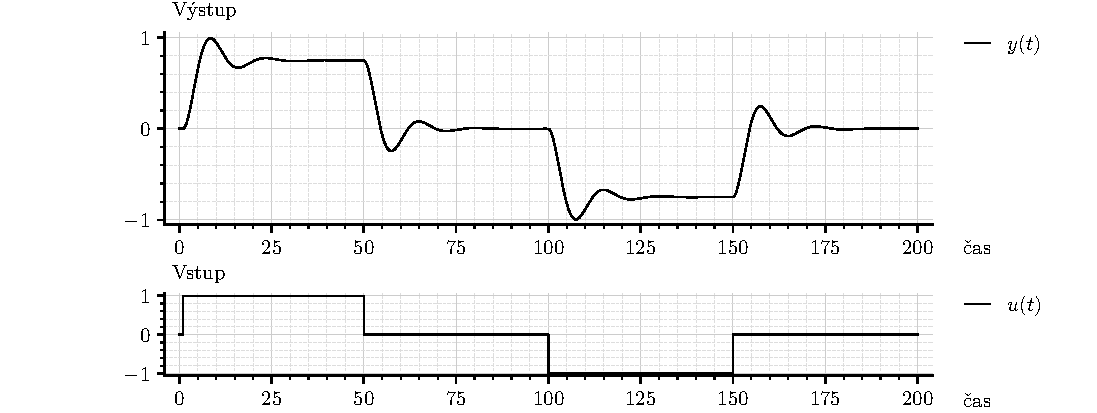
\includegraphics{figsc_ar03_fig01_1.pdf}
	}

    \vspace{-2mm}

    \figcaption{}

    \vspace{2mm}

    \label{figsc_ar03_fig01_0}

\end{centering}



















\subsection{Doplnenie algoritmu RMNŠ do simulačnej schémy}


V predchádzajúcom bola vytvorená simulačná schéma pre simuláciu uvažovaného riadeného systému. Tu je cieľom doplniť do simulačnej schémy algoritmus RMNŠ.

Pre úplnosť, ARX (AutoRegressive eXogenous) model, ktorý je identifikovaný (klasickou RMNŠ), je vo všeobecnosti nasledovný:
\begin{equation}
	A(z^{-1})y(k) = B(z^{-1})u(k) + \xi(k)
\end{equation}
kde
\begin{equation}
	\begin{split}
		 B(z^{-1}) &= b_1z^{-1} + \ldots + b_{n_b}z^{-n_b} \\
		 A(z^{-1}) &= 1 + a_1z^{-1} + \ldots + a_{n_a}z^{-n_a}
	\end{split}
\end{equation}
a $\xi(k)$ predstavuje poruchy a šum. V ďalšom budeme uvažovať $\xi(k) = 0$. ARX model vyjadrený v tvare diferenčnej rovnice:
\begin{equation}
	\begin{split}
		y(k) = & -a_1y(k-1) - \ldots - a_{n_a}y(k-n_a) +  b_1u(k-1) + \ldots + b_{n_b}u(k-n_b)
	\end{split}
\end{equation}


Nech modelom riadeného systému je diferenčná rovnica v uvedenom tvare, kde hodnoty $n_a = 2$ a $n_b = 2$. Potom táto diferenčná rovnica má tvar
\begin{equation}
	y(k) =  - a_1y(k-1) - a_2y(k-2) + b_1u(k-1) + b_2u(k-2)
\end{equation}

V maticovom zápise:
\begin{equation}
	y(k) = h^\mathsf T \Theta
\end{equation}
kde $h^\mathsf T = \begin{bmatrix} -y(k-1) & -y(k-2) & u(k-1) & u(k-2) \end{bmatrix}$  a $\Theta = \begin{bmatrix} a_1 & a_2 & b_1 & b_2 \end{bmatrix}^\mathsf T$.
Neznámymi parametrami modelu teda sú koeficienty $a_1$, $a_2$, $b_1$ a $b_2$.


\bigskip

\noindent
Takpovediac diferenciálne rovnice riadeného systému ostavajú samozrejme rovnaké ako sme ich realizovali v predchádzajúcom, teda aj tu („na začiatku skriptu“) platí výpis kódu~\ref{vypkparam} a \ref{vypkdr}.

\bigskip




\noindent
Simulačnú schému nech realizuje nasledujúca funkcia:

{\catcode`\-=12
\lstinputlisting[language=Python,
                 caption={Súbor \lstinline{ar03_pr02.py}},
                 % label={vypk01},
				 consecutivenumbers=false,
				 linerange=c02-c02,
                 ]{../../PY/ar03_pr02.py}
}


V uvedenej simulačnej schéme je implementovaný RMNŠ algoritmus, ktorého výstupom je vektor parametrov \lstinline{theta_k} a následne je tiež vypočítaná (v každom cykle) jednokroková predikcia výstupného signálu zapisovaná do vektora \lstinline{RMNS_y_predict_log}.

Všimnime si tiež napríklad, že faktor zabúdania $\lambda$ (premenná \lstinline{lambdaKoef}) je nastavený na hodnotu $\lambda = 1$, teda algoritmus nevyužíva zabúdanie.

Nastavenia potrebné pre samotnú simuláciu a vygenerovanie signálov, ktoré sa používajú pri simulácii (ktoré sú dopredu známe - dané):


{\catcode`\-=12
\lstinputlisting[language=Python,
                 caption={Súbor \lstinline{ar03_pr02.py}},
                 % label={vypk01},
				 consecutivenumbers=false,
				 linerange=c03-c03,
                 ]{../../PY/ar03_pr02.py}
}

\noindent
Pre simuláciu je potrebné vytvoriť vstupný signál $u(t)$ pre riadený systém. Nech je nasledovný:

{\catcode`\-=12
\lstinputlisting[language=Python,
                 caption={Súbor \lstinline{ar03_pr02.py}},
                 % label={vypk01},
				 consecutivenumbers=false,
				 linerange=c04-c04,
                 ]{../../PY/ar03_pr02.py}
}


\noindent
Spustenie simulácie:

{\catcode`\-=12
\lstinputlisting[language=Python,
                 caption={Súbor \lstinline{ar03_pr02.py}},
                 % label={vypk01},
				 consecutivenumbers=false,
				 linerange=c05-c05,
                 ]{../../PY/ar03_pr02.py}
}


\noindent
Nakreslenie obrázku (pre prehľadnosť je kód v samostatnom súbore):


{\catcode`\-=12
\lstinputlisting[language=Python,
                 caption={Súbor \lstinline{ar03_pr02.py}},
                 % label={vypk01},
				 consecutivenumbers=false,
				 linerange=c06-c06,
                 ]{../../PY/ar03_pr02.py}
}



\begin{centering}

	\makebox[\textwidth][c]{%
	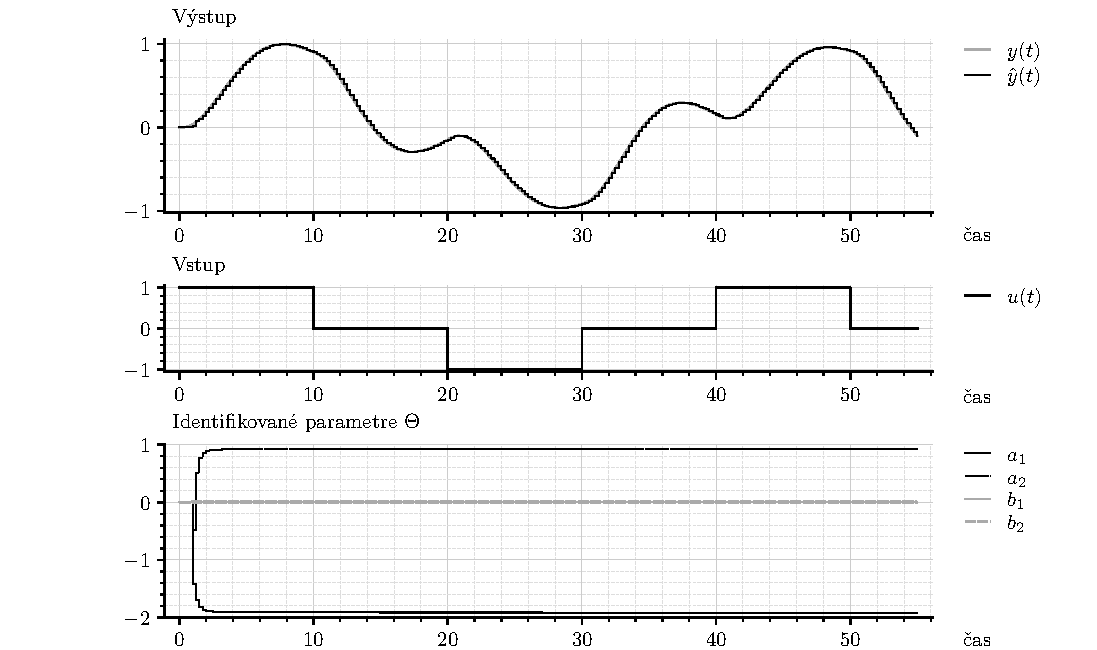
\includegraphics{figsc_ar03_fig02_0.pdf}
	}

    \vspace{-2mm}

    \figcaption{}

    \vspace{2mm}

    \label{figsc_ar03_fig02_0}

\end{centering}


Pre zaujímavosť, priebežne identifikované parametre $\Theta$ sú zapisované do poľa \lstinline{RMNS_theta_log}. Posledný riadok v tomto poli je:

{\catcode`\-=12
\lstinputlisting[language=Python,
                 caption={Súbor \lstinline{ar03_pr02.py}},
                 % label={vypk01},
				 consecutivenumbers=false,
				 linerange=c07-c07,
                 ]{../../PY/ar03_pr02.py}
}


\begin{lstlisting}[numbers=none]
[-1.91569536  0.92772642  0.00456786  0.00445568]
\end{lstlisting}








\subsection{Algoritmus RMNŠ pri zašumených dátach}

V predchádzajúcom bola vytvorená simulačná schéma pre simuláciu uvažovaného riadeného systému a bol do nej doplnený algoritmus RMNŠ.

Výstupná veličina samotného simulovaného riadeného systému je, pochopiteľne, bez šumu. Tu je cieľom preskúmať ako je RMNŠ schopný vysporiadať sa s prítomnosťou šumu v dátach výstupnej veličiny.



\bigskip

\noindent
Aj tu platí, že diferenciálne rovnice riadeného systému ostávajú samozrejme rovnaké ako sme ich realizovali v predchádzajúcom, teda aj tu („na začiatku skriptu“) platí výpis kódu~\ref{vypkparam} a \ref{vypkdr}.

\bigskip


\noindent
Simulačnú schému nech realizuje nasledujúca funkcia:

{\catcode`\-=12
\lstinputlisting[language=Python,
                 caption={Súbor \lstinline{ar03_pr03.py}},
                 % label={vypk01},
				 consecutivenumbers=false,
				 linerange=c02-c02,
                 ]{../../PY/ar03_pr03.py}
}

V uvedenej simulačnej schéme je implementovaný RMNŠ algoritmus, ktorého výstupom je vektor parametrov \lstinline{theta_k} a následne je tiež vypočítaná (v každom cykle) jednokroková predikcia výstupného signálu zapisovaná do vektora \lstinline{RMNS_y_predict_log}.

Nastavenia potrebné pre samotnú simuláciu a vygenerovanie signálov, ktoré sa používajú pri simulácii (ktoré sú dopredu známe - dané):

{\catcode`\-=12
\lstinputlisting[language=Python,
                 caption={Súbor \lstinline{ar03_pr03.py}},
                 % label={vypk01},
				 consecutivenumbers=false,
				 linerange=c03-c03,
                 ]{../../PY/ar03_pr03.py}
}

\noindent
Pre simuláciu je potrebné vytvoriť vstupný signál $u(t)$ pre riadený systém. Nech je nasledovný:


{\catcode`\-=12
\lstinputlisting[language=Python,
                 caption={Súbor \lstinline{ar03_pr03.py}},
                 % label={vypk01},
				 consecutivenumbers=false,
				 linerange=c04-c04,
                 ]{../../PY/ar03_pr03.py}
}


\subsubsection{Bez zabúdania}

Ďalším nastavením, špeciálne dôležitým v tomto príklade je koeficient zabúdania $\lambda$:

{\catcode`\-=12
\lstinputlisting[language=Python,
                 caption={Súbor \lstinline{ar03_pr03.py}},
                 % label={vypk01},
				 consecutivenumbers=false,
				 linerange=c04l-c04l,
                 ]{../../PY/ar03_pr03.py}
}

\noindent
Pamätajme teda, že faktor zabúdania $\lambda$ (premenná \lstinline{lambdaKoef}) je tu nastavený na hodnotu $\lambda = 1$, teda algoritmus nevyužíva zabúdanie.


\noindent
Spustenie simulácie:

{\catcode`\-=12
\lstinputlisting[language=Python,
                 caption={Súbor \lstinline{ar03_pr03.py}},
                 % label={vypk01},
				 consecutivenumbers=false,
				 linerange=c05-c05,
                 ]{../../PY/ar03_pr03.py}
}

\noindent
Nakreslenie obrázka (pre prehľadnosť je kód v samostatnom súbore):

{\catcode`\-=12
\lstinputlisting[language=Python,
                 caption={Súbor \lstinline{ar03_pr03.py}},
                 % label={vypk01},
				 consecutivenumbers=false,
				 linerange=c06-c06,
                 ]{../../PY/ar03_pr03.py}
}



\begin{centering}

	\makebox[\textwidth][c]{%
	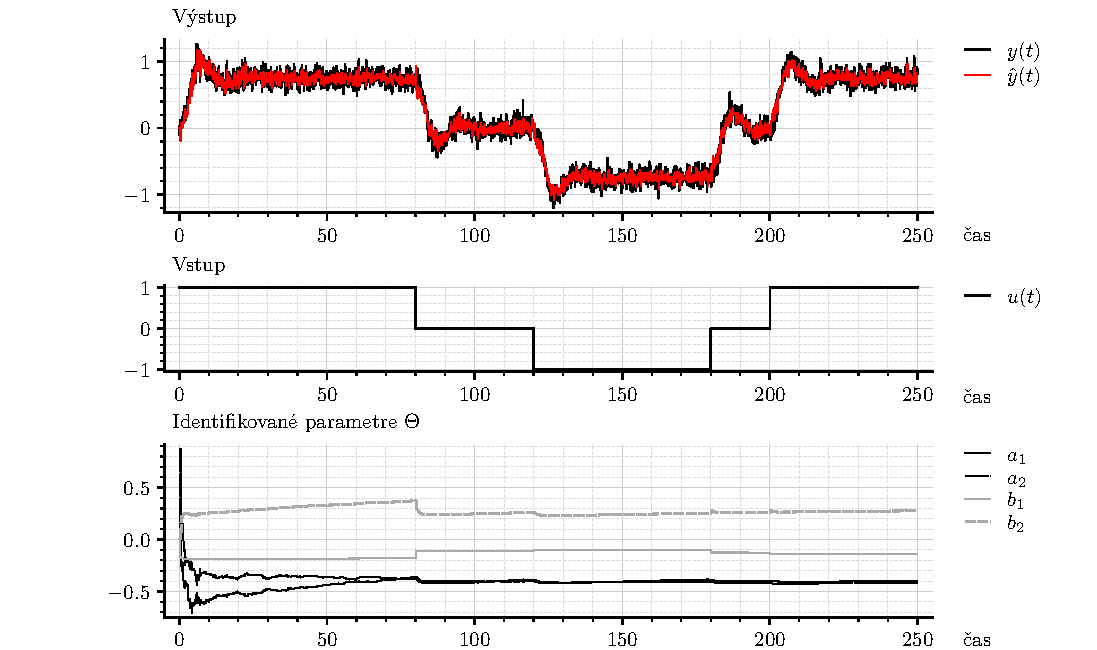
\includegraphics{figsc_ar03_fig03_0.pdf}
	}

    \vspace{-2mm}

    \figcaption{}

    \vspace{2mm}

    \label{figsc_ar03_fig03_0}

\end{centering}








\subsubsection{So zabúdaním}


Iná simulácia nech je s nasledovným koeficientom zabúdania:


{\catcode`\-=12
\lstinputlisting[language=Python,
                 caption={Súbor \lstinline{ar03_pr03.py}},
                 % label={vypk01},
				 consecutivenumbers=false,
				 linerange=c07-c07,
                 ]{../../PY/ar03_pr03.py}
}



\begin{centering}

	\makebox[\textwidth][c]{%
	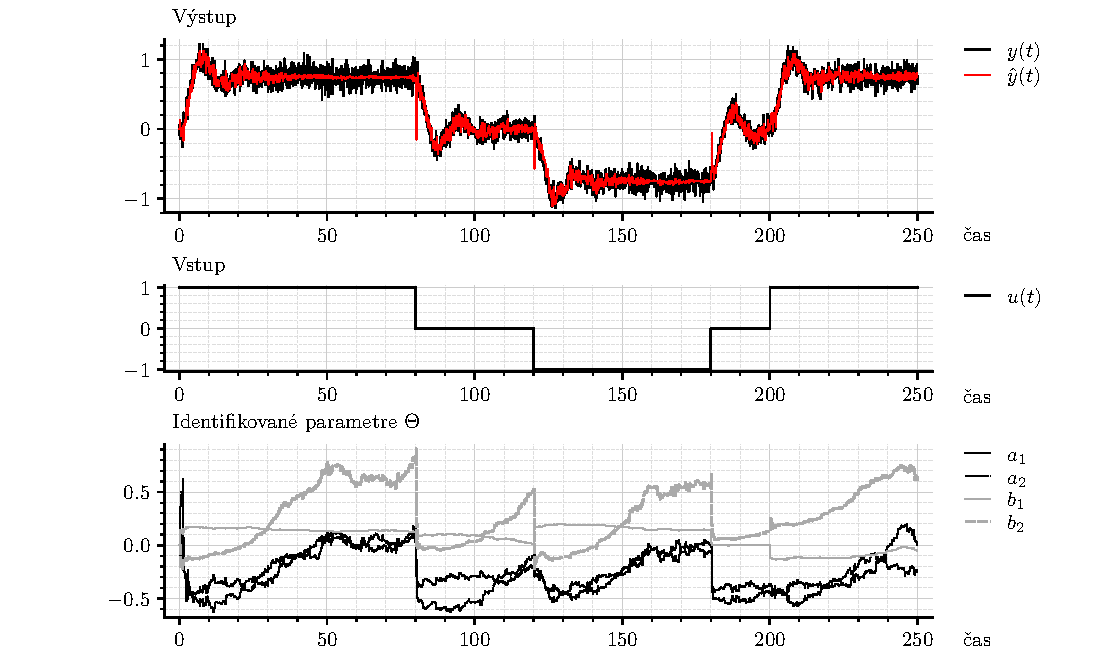
\includegraphics{figsc_ar03_fig03_1.pdf}
	}

    \vspace{-2mm}

    \figcaption{}

    \vspace{2mm}

    \label{figsc_ar03_fig03_1}

\end{centering}










\noindent
Extrémnou voľbou koeficientu zabúdania pre tento prípad by bolo:


{\catcode`\-=12
\lstinputlisting[language=Python,
                 caption={Súbor \lstinline{ar03_pr03.py}},
                 % label={vypk01},
				 consecutivenumbers=false,
				 linerange=c08-c08,
                 ]{../../PY/ar03_pr03.py}
}



\begin{centering}

	\makebox[\textwidth][c]{%
	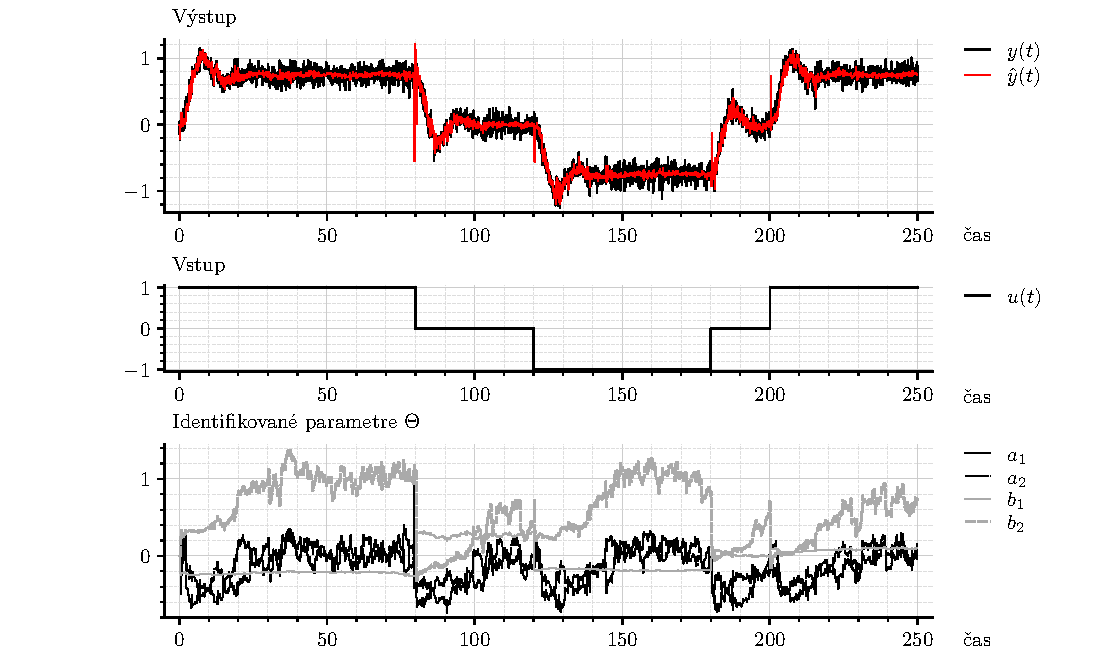
\includegraphics{figsc_ar03_fig03_2.pdf}
	}

    \vspace{-2mm}

    \figcaption{}

    \vspace{2mm}

    \label{figsc_ar03_fig03_2}

\end{centering}


































\subsection{Iná ukážka simulačnej schémy pre simuláciu RMNŠ}

V tejto časti sa použije Simulink pre riešenie úloh ako v predchádzajúcom.

\medskip

\noindent
Majme sústavu, lepšie povedané dynamický systém (ktorý neskôr budeme riadiť), a~k~tomu istý blok, ktorého funkciou je realizovať priebežnú identifikáciu predmetného systému. Schematicky znázornené:


\begin{centering}

	\makebox[\textwidth][c]{%
	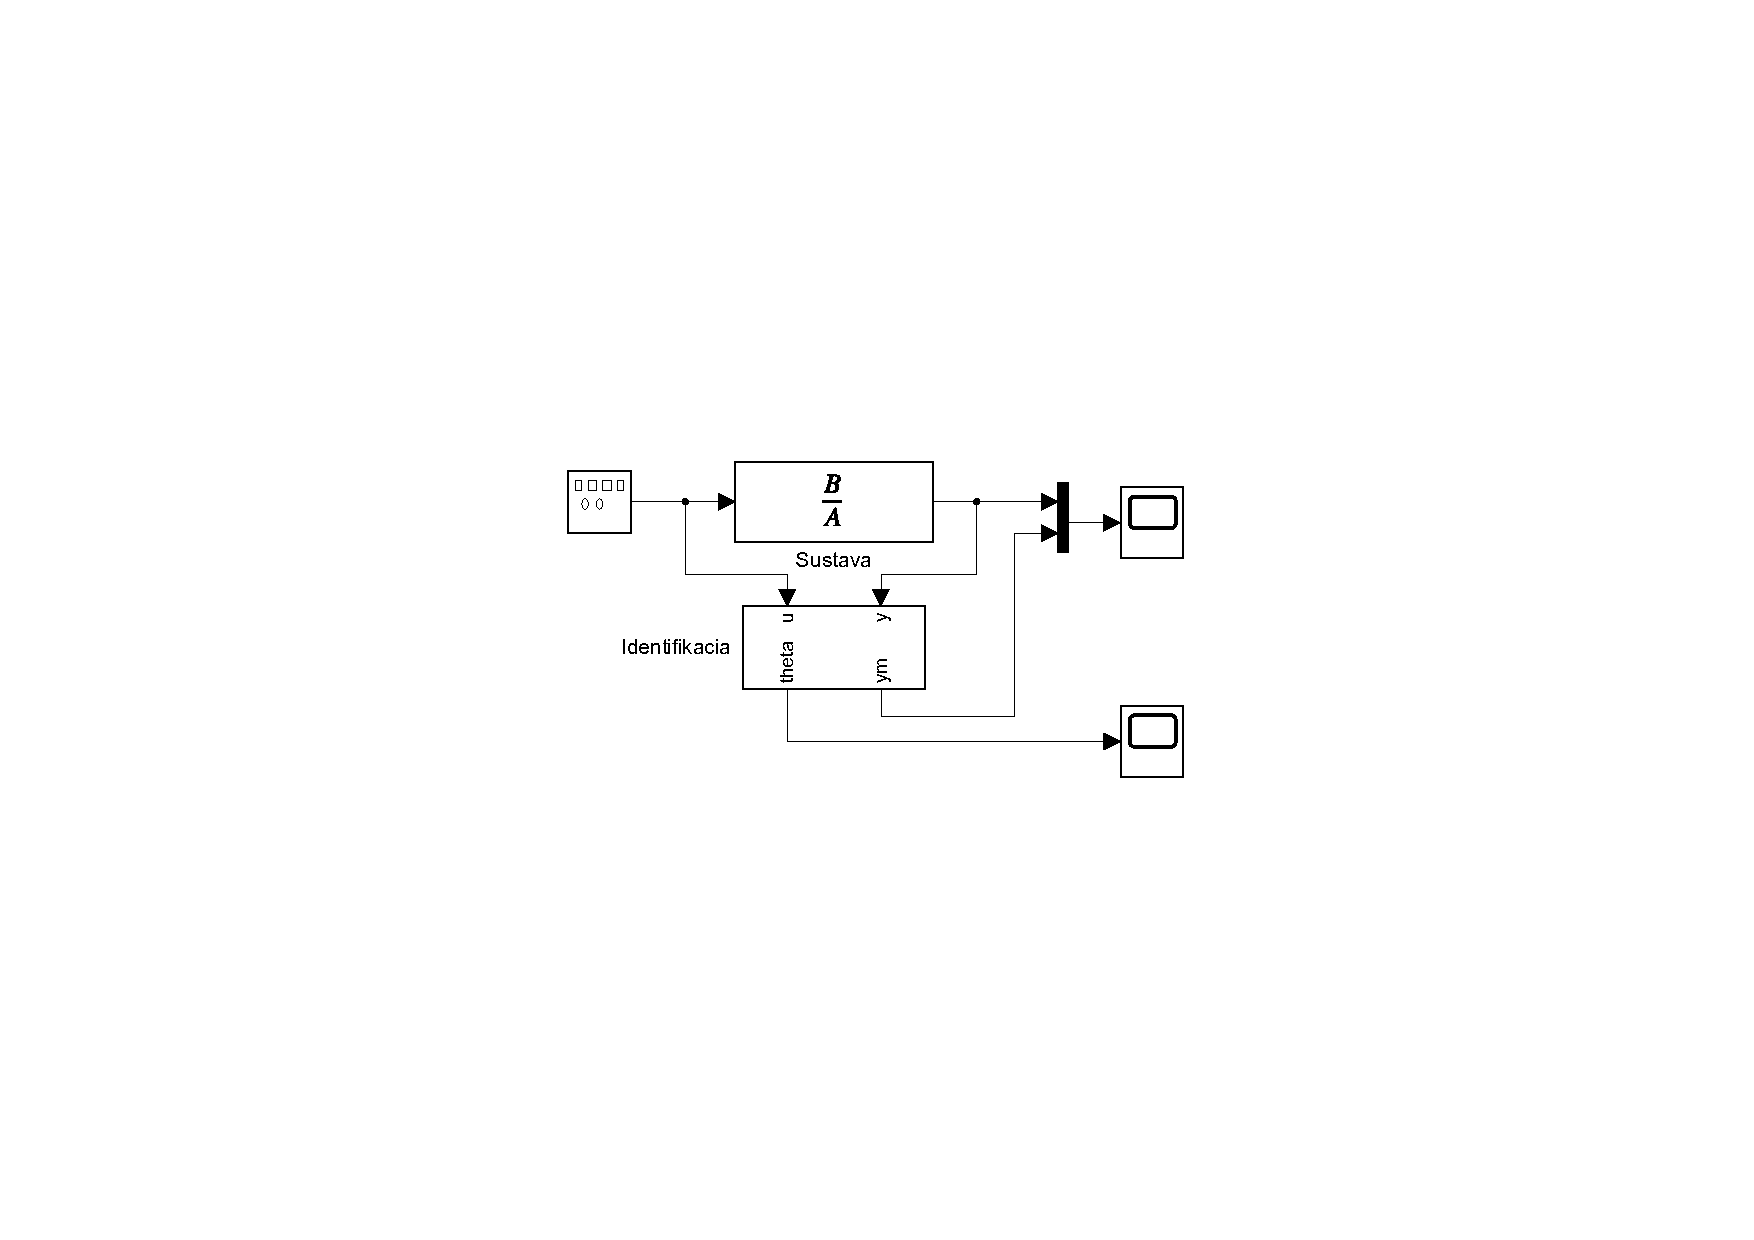
\includegraphics[viewport=85mm 75mm 205mm 138mm, clip, scale=0.9]{ar03_sim_RMNS.pdf}
	}

    \vspace{-2mm}

    \figcaption{}

    \vspace{2mm}

    \label{sim_RMNS}

\end{centering}


\noindent
Blok Identifikácia slúži na priebežnú identifikáciu a teda jeho hlavným výstupom sú parametre $\Theta$ a tiež sa uvažuje výstupná veličina modelu $\hat y$ (na obr. označená ako \lstinline{ym}).

Pred spustením schémy (v Simulinku) je samozrejme potrebné inicializovať parametre riadeného systému (sústavy) a ako sa ukáže aj iné veci (v tomto prípade). Je to realizované v skripte:
{\catcode`\-=12
\lstinputlisting[language=Matlab,
                 caption={Súbor \lstinline{ar03_spustima_RMNS.m}},
                 % label={vypk01},
                 ]{../../ML/ar03_spustima_RMNS.m}
}



\noindent
Samotný blok Identifikácia je realizovaný nasledovne:


\begin{centering}

	\makebox[\textwidth][c]{%
	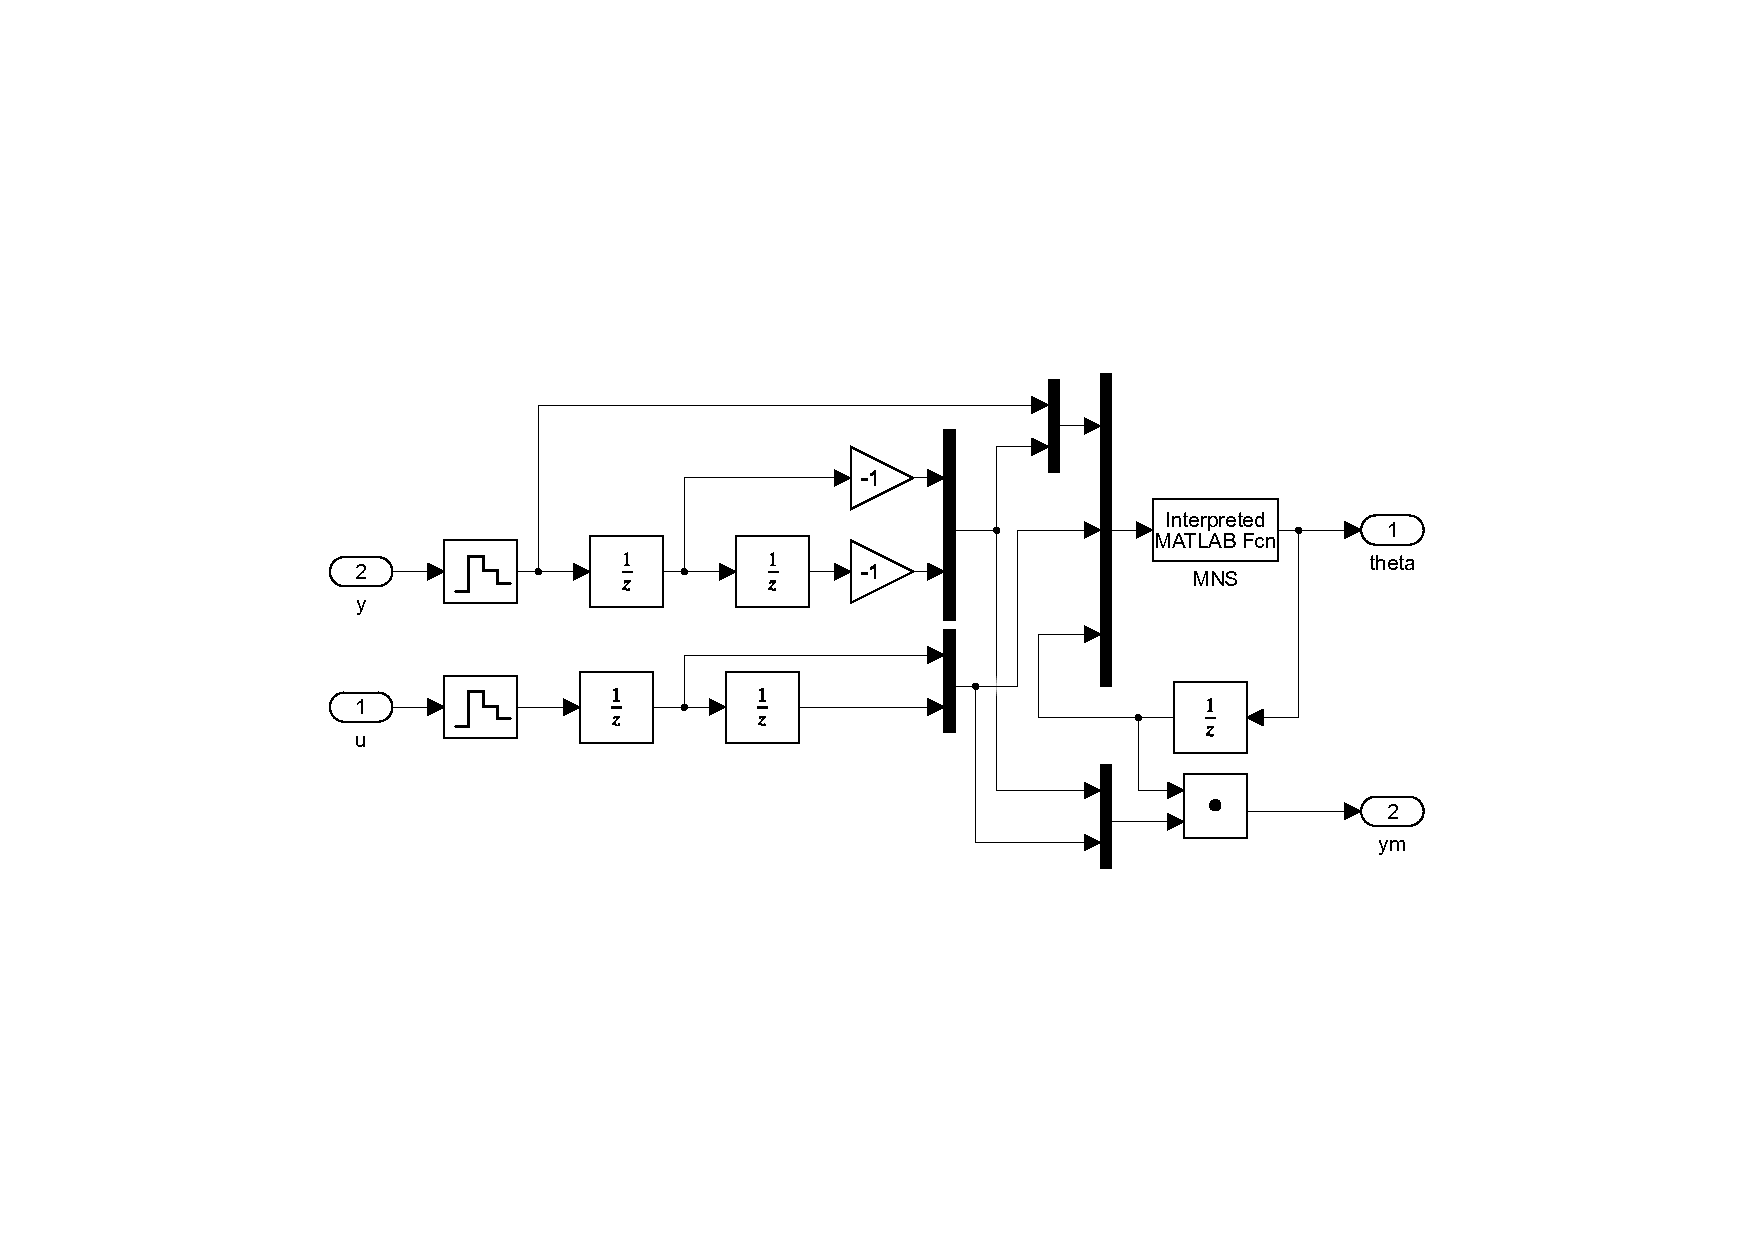
\includegraphics[viewport=50mm 60mm 245mm 150mm, clip, scale=0.9]{Identifikacia.pdf}
	}

    \vspace{-2mm}

    \figcaption{}

    \vspace{2mm}

    \label{Identifikacia}

\end{centering}


\noindent
Obsahuje vzorkovanie signálov (zero order hold) a oneskorovanie signálov (v zmysle $z^{-1}$). Tým je realizované získavanie tzv. signálneho vektora a podobne. Ďalej je súčasťou bloku funkcia, ktorá realizuje samotný algoritmus RMNŠ. Kód funkcie:

{\catcode`\-=12
\lstinputlisting[language=Matlab,
                 caption={Súbor \lstinline{MNS.m}},
                 % label={vypk01},
                 ]{../../ML/MNS.m}
}
























\section{Metóda rozmiestňovania pólov}




Pripomeňme, že zákon riadenia (štruktúra riadenia) samonastavujúceho sa regulátora v~uvažovanom konkrétnom príklade je v tvare
\begin{subequations} \label{zakonRiadenia2}
	\begin{align}
		R(z^{-1})u(k) & = T(z^{-1})r(k) - S(z^{-1})y(k) \\
		u(k) & = \frac{T(z^{-1})}{R(z^{-1})}r(k) - \frac{S(z^{-1})}{R(z^{-1})}y(k)
	\end{align}
\end{subequations}
kde $R$, $S$ a $T$ sú polynómy v tvare
\begin{subequations}
	\begin{align}
		R(z^{-1}) & = 1 + r_1z^{-1} + r_2z^{-2} + \ldots +  r_{n_r}z^{-n_r}\\
		S(z^{-1}) & = s_0 + s_1z^{-1} + s_2z^{-2} + \ldots +  s_{n_s}z^{-n_s} \\
		T(z^{-1}) & = t_0 + t_1z^{-1} + t_2z^{-2} + \ldots +  t_{n_t}z^{-n_t}
	\end{align}
\end{subequations}
Ako už bolo uvedené, koeficienty polynómov sú parametrami regulátora. Počet parametrov regulátora závisí od stupňa jednotlivých polynómov. Pre uvažovaný konkrétny príklad sú stupne polynómov nasledovné: $n_r = 1$, $n_s = 1$ a $n_t = 0$. Potom počet parametrov regulátora je $n_r + n_s + 1 + n_t + 1$. Teda $1 + 1 + 1 + 0 + 1 = 4$. Zákon riadenia je možné zapísať aj v tvare diferenčnej rovnice:
\begin{equation}
	u(k) =  - r_1 u(k-1) - s_0 y(k) - s_1 y(k-1) + t_0 r(k)
\end{equation}


\bigskip

Uvažujme zákon riadenia v tvare \eqref{zakonRiadenia2}, ktorého parametre budeme počítať pomocou metódy rozmiestňovania pólov. Najprv odvodíme rovnicu uzavretého obvodu (URO).



















\subsection{Rovnica URO}


Model riadeného systému je
\begin{equation} \label{modelRiadSys}
	A(z^{-1})y(k)
	=
		B(z^{-1})u(k)
\end{equation}
Dosadením \eqref{zakonRiadenia} do \eqref{modelRiadSys} máme
\begin{equation}
	A(z^{-1})y(k) = B(z^{-1}) \left( \frac{T(z^{-1})}{R(z^{-1})}r(k) - \frac{S(z^{-1})}{R(z^{-1})}y(k) \right)
\end{equation}
Úpravou
\begin{subequations}
	\begin{align}
		A y(k) &= \frac{BT}{R} r(k) - \frac{BS}{R} y(k) \\
		RA y(k) &= BT r(k) - BS y(k)\\
		\left( RA + BS \right) y(k) &= BT r(k) \\
		y(k) &= \frac{BT}{\left( AR + BS \right)} r(k) \\
		\frac{y(k)}{r(k)} &= \frac{BT}{\left( AR + BS \right)}
	\end{align}
\end{subequations}
Charakteristický polynóm uzavretého regulačného obvodu je:
\begin{equation}
	A(z^{-1})R(z^{-1}) + B(z^{-1})S(z^{-1})
\end{equation}


Nech želaný polynóm je
\begin{equation}
	P(z^{-1})  = 1 + p_1z^{-1} + p_2z^{-2} + \ldots +  p_{n_p}z^{-n_p}
\end{equation}
potom diofantická rovnica, z ktorej sa vypočítajú koeficienty polynómov $R$ a $S$ je
\begin{equation} \label{prvaDiofantRovn}
	A(z^{-1})R(z^{-1}) + B(z^{-1})S(z^{-1})  = 	P(z^{-1})
\end{equation}




V tomto prípade máme
\begin{subequations}
	\begin{align}
		A & = 1 + a_1z^{-1} + a_2z^{-2} \\
		B & = b_1z^{-1} + b_2z^{-2} \\
		R & = 1 + r_1z^{-1} \\
		S & = s_0 + s_1z^{-1}
	\end{align}
\end{subequations}
a nech želaný polynóm pre tento prípad je
\begin{equation}
	\begin{split}
		P & = 1 + p_1z^{-1} + p_2z^{-2}
	\end{split}
\end{equation}
Diofantická rovnica pre tento prípad
\begin{equation}
	\begin{split}
		& \left( 1 + a_1z^{-1} + a_2z^{-2} \right) \left( 1 + r_1z^{-1} \right) + \left( b_1z^{-1} + b_2z^{-2} \right) \left( s_0 + s_1z^{-1} \right) \\
		&= 1 + p_1z^{-1} + p_2z^{-2}
	\end{split}
\end{equation}
Roznásobením
\begin{equation}
	\begin{split}
		& 1+r_1z^{-1}+a_1z^{-1} + a_1r_1z^{-2}+a_2z^{-2}+a_2r_1z^{-3} \\
		&+ b_1s_0z^{-1}+b_1s_1z^{-2} + b_2s_0z^{-2}+b_2s_1z^{-3} \\
		&= 1 + p_1z^{-1} + p_2z^{-2}
	\end{split}
\end{equation}
Na ľavej strane ponecháme členy, v ktorých sa nachádzajú neznáme koeficienty polynómov zo zákona adaptácie a ostatné členy presunieme na pravú stranu
\begin{equation}
	\begin{split}
		& r_1z^{-1} + a_1r_1z^{-2}+a_2r_1z^{-3} + b_1s_0z^{-1}+b_1s_1z^{-2} + b_2s_0z^{-2}+b_2s_1z^{-3} \\
		&= 1 + p_1z^{-1} + p_2z^{-2} - 1 -a_1z^{-1} -a_2z^{-2}
	\end{split}
\end{equation}
Po úprave
\begin{equation}
	\begin{split}
		& \left({ r_1 + b_1s_0 }\right) z^{-1} + \left({ a_1r_1 +b_1s_1 + b_2s_0 }\right) z^{-2} + \left({ a_2r_1 +b_2s_1 }\right) z^{-3} \\
		&= \left({ p_1 -a_1 }\right) z^{-1} + \left({p_2 -  a_2 }\right) z^{-2}
	\end{split}
\end{equation}
Porovnaním koeficientov pri rovnakých mocninách získame rovnice
\begin{subequations}
	\begin{align}
		 r_1 + b_1 s_0  &= p_1 - a_1 \\
		 a_1 r_1 + b_2 s_0 + b_1 s_1  &= p_2 -  a_2 \\
		 a_2 r_1  + b_2 s_1  &= 0
	\end{align}
\end{subequations}
V maticovom zápise:
\begin{equation}
	\begin{bmatrix} 1 & b_1 & 0 \\ a_1 & b_2 & b_1 \\ a_2 &   0 & b_2 \end{bmatrix}
	\begin{bmatrix} r_1 \\ s_0 \\ s_1  \end{bmatrix}
	=
	\begin{bmatrix} p_1 - a_1 \\ p_2 - a_2 \\ 0 \end{bmatrix}
\end{equation}






Maticový zápis vyplývajúci z diofantickej rovnice v prípade, keď stupne polynómov $R$, $S$ a $P$ sú všeobecné, je v tvare
\begin{equation} \label{VelkaDiofanRov}
	\begin{bmatrix}
		   1 &      0 &      0 & \cdots &       0 &     b_1 &      0 &      0 & \cdots &       0 \\
	 	 a_1 &      1 &      0 & \cdots &       0 &     b_2 &    b_1 &      0 & \cdots &       0 \\
	 	 a_2 &    a_1 &      1 & \cdots &       0 &     b_3 &    b_2 &    b_1 & \cdots &       0 \\
      \vdots & \vdots & \vdots & \ddots &  \vdots &  \vdots & \vdots & \vdots & \ddots &  \vdots \\
     a_{n_a} & \vdots & \vdots & \cdots &       1 & b_{n_b} & \vdots & \vdots & \cdots &     b_1 \\
           0 & \ddots & \vdots & \cdots &     a_1 &       0 & \ddots & \vdots & \cdots &  \vdots \\
      \vdots & \vdots & \ddots & \cdots &  \vdots &  \vdots & \vdots & \ddots & \cdots &  \vdots \\
      \vdots & \vdots & \vdots & \ddots &  \vdots &  \vdots & \vdots & \vdots & \ddots &  \vdots \\
           0 &      0 &      0 & \cdots & a_{n_a} &       0 &      0 &      0 & \cdots & b_{n_b}
	\end{bmatrix}
	\begin{bmatrix} r_1 \\ r_2 \\ r_2 \\ \vdots \\ r_{n_r} \\ s_0 \\ s_1 \\ s_2 \\ \vdots \\ s_{n_s} \end{bmatrix}
	=
	\begin{bmatrix} p_1 - a_1 \\ p_2 - a_2 \\ \vdots \\ 0 \\ \vdots \\ 0 \end{bmatrix}
\end{equation}


Takáto sústava rovníc bude mať riešenie ak
\begin{subequations}
	\begin{align}
		 n_r &= n_b - 1 \\
		 n_s &= n_a - 1
	\end{align}
\end{subequations}







\subsection{Polynóm $T$}

\bigskip

Zatiaľ sme vypočítali koeficienty polynómov $R$ a $S$. Otázkou ostáva, ako určiť polynóm $T$. Je potrebné určiť jeho stupeň a vypočítať koeficienty. V úvode sme \uv{zvolili}, že stupeň polynómu $T$ je $n_t = 0$. Teda jediným koeficientom bude $t_0$. Ukážme teraz, že jednou z možností, ako určiť polynóm $T$, je žiadať nulovú regulačnú odchýlku v ustálenom stave. Dostaneme tak polynóm $T$ práve nultého stupňa a aj výpočet koeficientu $t_0$.

Keďže charakteristická rovnica URO je rovnaká ako želaný polynóm $P$, je možné písať rovnicu uzavretého obvodu v tvare
\begin{equation}
	y(k) = \frac{BT}{P} r(k)
\end{equation}
Aby platilo
\begin{equation}
	y(\infty) = r(\infty)
\end{equation}
musí byť
\begin{subequations}
	\begin{align}
		BT &= P \\
		T &= \frac{P}{B}
	\end{align}
\end{subequations}
A keďže \uv{donekonečna} je v diskrétnej doméne \uv{dojednotky}, teda $z = 1$, potom
\begin{equation}
	T = \frac{P(1)}{B(1)}
\end{equation}
čo v tomto prípade znamená
\begin{equation}
	T(z^{-1}) = \frac{1 + p_1 + p_2}{b_1 + b_2} = t_0
\end{equation}





\subsubsection{Alternatívy spôsob určenia polynómu $T$}

\paragraph{Alternatíva 1}

Ďalší spôsob ako určiť koeficienty polynómu $T$ je nasledovný. Nájdeme obraz referenčného signálu tak, že jeho časovú formu pretransformujeme pomocou Z-transformácie. Totiž v mnohých prípadoch je možné dopredu určiť časový priebeh referenčného signálu a~navyše sa referenčný signál skladá zo skokov, rámp a~podobných, pomocou Z-transformácie, ľahko transformovateľných signálov. Obraz referenčného signálu je
\begin{equation}
	\left\{ r(t) \right\}_q = \frac{F \left( q^{-1} \right)}{G \left( q^{-1} \right)}
\end{equation}
Tento obraz použijeme vo vzťahu pre regulačnú odchýlku:
\begin{equation}
	e = r - y = r - \frac{BT}{P}r = \frac{F}{G} - \frac{BT}{P}\frac{F}{G} = \frac{F(P - BT)}{GP} = \frac{FN}{P}
\end{equation}
kde sme označili
\begin{equation}
	\frac{P - BT}{G} = N
\end{equation}
Z tohto označenia môžeme písať diofantickú rovnicu, ktorá doplní \eqref{prvaDiofantRovn}, a vznikne tak sústava.
\begin{equation}
	GN + BT = P
\end{equation}
Z tejto rovnice sa dá určiť aj polynóm vyššieho ako nultého stupňa.



\paragraph{Alternatíva 2}

Ďalší spôsob ako určiť koeficienty polynómu $T$ je takýto: ak bude polynóm $T$~obrátenou hodnotou polynómu $B$, teda $T = 1/B$, zaistí sa tak nie len nulová regulačná odchýlka v ustálenom stave, ale aj to, že polynóm $B$ nebude mať žiadny vplyv na dynamiku URO. Dynamika URO bude daná len želaným charakteristickým polynómom $P$, takto:
\begin{equation}
	y(t) = \frac{1}{P}r(t)
\end{equation}
Zákon riadenia potom môžeme uvažovať v tvare
\begin{equation}
	Ru(t) = \frac{1}{B}r(t) - Sy(t) \quad \Rightarrow \quad r = BRu + BSy
\end{equation}
Ale ak $B = q^{-D}\tilde{B}$, tak aby sme mohli napísať predchádzajúcu rovnicu musíme dať $q^{-D}$ na druhú stranu k $r$. Teda:
\begin{equation}
	 rq^{D} = \tilde{B}Ru + \tilde{B}Sy
\end{equation}
Ak potom vyjadríme akčný zásah, je zrejmé, že bude závisieť od budúcich hodnôt referenčného signálu $u(t) = r(t + D)-\ldots$ Toto však nemusí byť prekážkou, pretože v mnohých prípadoch je referenčný signál dopredu známy.




\subsection{Súhrn pre tento prípad}

Zhrňme výpočty potrebné pre určenie parametrov regulátora pre tento prípad.

Hodnoty parametrov modelu $a_1$, $a_2$, $b_1$ a $b_2$ sú po identifikácii (v danej perióde vzorkovania) známe a prirodzene sú známe aj hodnoty koeficientov želaného polynómu $P$. Hodnoty parametrov regulátora získame riešením
\begin{equation}
	\begin{bmatrix} 1 & b_1 & 0 \\ a_1 & b_2 & b_1 \\ a_2 &   0 & b_2 \end{bmatrix}
	\begin{bmatrix} r_1 \\ s_0 \\ s_1  \end{bmatrix}
	=
	\begin{bmatrix} p_1 - a_1 \\ p_2 - a_2 \\ 0 \end{bmatrix}
\end{equation}
a
\begin{equation}
		t_0 = \frac{1 + p_1 + p_2}{b_1 + b_2}
\end{equation}
















\subsection{Rýchlostný algoritmus metódy rozmiestňovania pólov}

Táto subsekcia je tu len pre ilustráciu širších obzorov týkajúcich sa oblasti používania metódy rozmiesňovania pólov v prípadoch podobných tomuto.

\bigskip


\noindent
Keďže ide o rýchlostný algoritmus, je potrebné vyjadriť prírastok akčnej veličiny:
\begin{align}
	 \Delta u(t) &= u(t) - u(t-1) = (1 - q^{-1})u(t) \\
	 u(t) &= \frac{\Delta u(t)}{(1 - q^{-1})}
\end{align}
Riadený systém a jeho ARX model (s nulovým šumom):
\begin{equation}
	Ay(t) = Bu(t)
\end{equation}
do ktorého dosadíme $u(t)$ a upravíme\ldots
\begin{subequations}
	\begin{align}
		 Ay(t) &= B\frac{\Delta u(t)}{(1 - q^{-1})} \\
		 (1 - q^{-1})Ay(t) &= B\Delta u(t)
	\end{align}
\end{subequations}
Zákon riadenia uvažujeme v tvare:
\begin{equation}
	\Delta u(t) = \frac{S}{R}(r(t) - y(t))
\end{equation}
Rovnica URO potom bude mať tvar
\begin{subequations}
	\begin{align}
		 (1 - q^{-1})Ay(t) &= B\Delta u(t) \\
		 (1 - q^{-1})Ay(t) & = B \frac{S}{R}(r(t) - y(t)) \\
		 (1 - q^{-1})ARy(t) &= BS(r(t) - y(t)) \\
		 (1 - q^{-1})ARy(t) &= BSr(t) - BSy(t) \\
		 ((1-q^{-1})AR + BS) y(t) &= BSr(t) \\
		 y(t) &= \frac{BS}{(1-q^{-1})AR + BS}r(t)
	\end{align}
\end{subequations}
Takže charakteristický polynóm je
\begin{equation}
	P = \left( 1 - q^{-1} \right) AR + BS
\end{equation}
Ale veď potom
\begin{equation}
	BS = P - \left( 1 - q^{-1} \right)AR
\end{equation}
a tak rovnica URO:
\begin{subequations}
	\begin{align}
		y(t) &= \frac{P - (1-q^{-1})AR}{P}r(t) \\
		y(t) &=\left({\frac{P}{P} -  \frac{(1-q^{-1})AR}{P}}\right)r(t) \\
		y(t) &= r(t) -  \frac{(1-q^{-1})AR}{P}r(t)
	\end{align}
\end{subequations}
Ak sa teraz opýtame aká bude regulačná odchýlka v ustálenom stave t.j. $y(\infty)$, $r(\infty)$ a čo je najdôležitejšie $q = 1$ potom:
\begin{equation}
	\begin{split}
		& y(\infty) =r(\infty) -  \frac{(1-1)AR}{P}r(\infty)
		\\& y(\infty) =r(\infty)
	\end{split}
\end{equation}
Teda regulačná odchýlka v ustálenom stave bude nulová (pretože sa zhodujú hodnoty referenčného signálu a~výstupnej veličiny).











\section{Cvičenie tretie}
\label{cvictretie}


\begin{enumerate}[leftmargin=0pt, labelsep=4mm, itemsep=0pt]

	\item Zrealizujte (v simulačnom prostredí) samonastavujúci sa regulátor tak ako to predpokladá uvažovaný konkrétny príklad.

	Nech želaným charakteristickým polynómom (pre uvažovaný konkrétny príklad) je $P(z^{-1}) = 1 + p_1z^{-1} + p_2z^{-2}$ pričom $p_1 = -1,6$ a~$p_2 = 0,64$, teda dvojnásobný koreň $z_{1,2} = 0,8$.

	Alternatívne, nech v želanom charakteristickom je $p_1 = -0,8$ a~$p_2 = 0,16$, teda dvojnásobný koreň $z_{1,2} = 0,4$.

	Pozn: pre uvažovaný príklad sa odporúča perióda vzorkovania $T_{vz} = 0,1$ [čas].

\end{enumerate}



\subsection{Konkrétny príklad samonastavujúceho sa regulátora}


V predchádzajúcom bola prezentovaná simulačná schéma, v ktorej bol implementovaný algoritmus RMNŠ.

Tu je cieľom doplniť do simulačnej schémy výpočet, ktorý na základe priebežne identifikovaných parametrov riadeného systému vypočíta hodnoty parametrov daného zákona riadenia a následne vypočíta samotný akčný zásah.

Výpočet parametrov zákona riadenia využíva matódu rozmistňovania pólov URO a je dplnený výpočtom pre zabezpečenie nulovej trvalej regulačnej odchýlky.

Nech želaným charakteristickým polynómom (pre uvažovaný konkrétny príklad) je $P(z^{-1}) = 1 + p_1z^{-1} + p_2z^{-2}$ pričom $p_1 = -1,6$ a $p_2 = 0,64$, teda dvojnásobný koreň $z_{1,2} = 0,8$.

Pozn: pre uvažovaný príklad sa odporúča perióda vzorkovania $T_{vz} = 0,1$ [čas].




V tomto konkrétnom príklade uvažovaný zákon riadenia je možné zapísať v tvare diferenčnej rovnice:
\begin{equation}
	u(k) =  - r_1 u(k-1) - s_0 y(k) - s_1 y(k-1) + t_0 r(k)
\end{equation}

Hodnoty parametrov modelu $a_1$, $a_2$, $b_1$ a $b_2$ sú po identifikácii (v danej perióde vzorkovania) známe a prirodzene sú známe aj hodnoty koeficientov želaného polynómu $P$. Hodnoty parametrov regulátora získame riešením
\begin{equation}
	\begin{bmatrix} 1 & b_1 & 0 \\ a_1 & b_2 & b_1 \\ a_2 &   0 & b_2 \end{bmatrix}
	\begin{bmatrix} r_1 \\ s_0 \\ s_1  \end{bmatrix}
	=
	\begin{bmatrix} p_1 - a_1 \\ p_2 - a_2 \\ 0 \end{bmatrix}
\end{equation}
a
\begin{equation}
		t_0 = \frac{1 + p_1 + p_2}{b_1 + b_2}
\end{equation}


\bigskip

\noindent
Aj tu platí, že diferenciálne rovnice riadeného systému ostávajú samozrejme rovnaké ako sme ich realizovali v predchádzajúcom, teda aj tu („na začiatku skriptu“) platí výpis kódu~\ref{vypkparam} a \ref{vypkdr}.

\bigskip

\noindent
Ďalej nech simulačnú schému realizuje nasledujúca funkcia:

{\catcode`\-=12
\lstinputlisting[language=Python,
                 caption={Súbor \lstinline{ar03_pr04.py}},
                 % label={vypk01},
				 consecutivenumbers=false,
				 linerange=c02-c02,
                 ]{../../PY/ar03_pr04.py}
}


\noindent
V uvedenej simulačnej schéme je implementovaný RMNŠ algoritmus rovnako ako v~predchádzajúcom...

Všimnime si však, že faktor zabúdania $\lambda$ (premenná \lstinline{lambdaKoef}) je nastavený na hodnotu $\lambda = 0,95$.

Tiež je potrebné všimnúť si, že štartovacie hodnoty RMNŠ algoritmu sú:

\noindent
\lstinline{RMNS_theta_0 = np.array([[-1.5], [0.5], [-2e-5], [1.5e-3]])}

\noindent
a

\noindent
\lstinline{RMNS_P_0 = np.diag([10*2, 10**2, 10**5, 10**5])}

\noindent
Nastavenia potrebné pre samotnú simuláciu a vygenerovanie signálov, ktoré sa používajú pri simulácii (ktoré sú dopredu známe - dané):


{\catcode`\-=12
\lstinputlisting[language=Python,
                 caption={Súbor \lstinline{ar03_pr04.py}},
                 % label={vypk01},
				 consecutivenumbers=false,
				 linerange=c03-c03,
                 ]{../../PY/ar03_pr04.py}
}

\noindent
Spustenie simulácie:


{\catcode`\-=12
\lstinputlisting[language=Python,
                 caption={Súbor \lstinline{ar03_pr04.py}},
                 % label={vypk01},
				 consecutivenumbers=false,
				 linerange=c05-c05,
                 ]{../../PY/ar03_pr04.py}
}

\noindent
Nakreslenie obrázka:

{\catcode`\-=12
\lstinputlisting[language=Python,
                 caption={Súbor \lstinline{ar03_pr04.py}},
                 % label={vypk01},
				 consecutivenumbers=false,
				 linerange=c06-c06,
                 ]{../../PY/ar03_pr04.py}
}

\begin{centering}

	\makebox[\textwidth][c]{%
	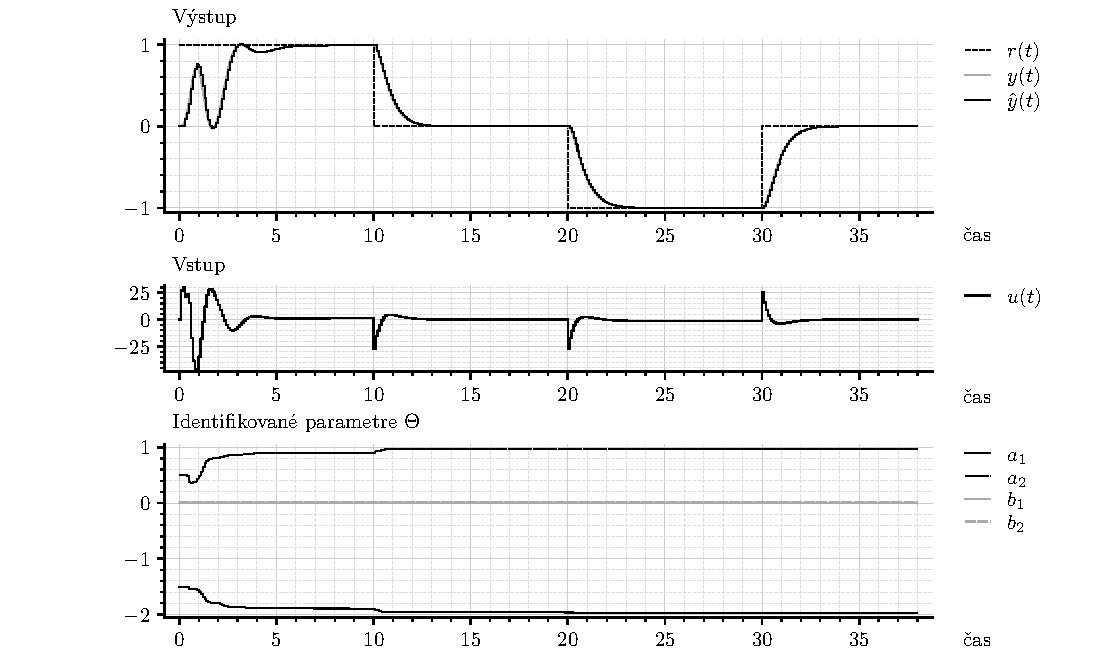
\includegraphics{figsc_ar03_fig04_0.pdf}
	}

    \vspace{-2mm}

    \figcaption{}

    \vspace{2mm}

    \label{figsc_ar03_fig04_0}

\end{centering}




















\subsection{Simulácia v Simulinku}



V tejto časti sa použije Simulink pre riešenie úloh ako v predchádzajúcom.

\medskip

\noindent
Máme riadený systém, ku ktorému sme v predchádzajúcom vyrobili blok pre priebežnú identifikáciu. Teraz pridajme blok, ktorý bude realizovať výpočet akčného zásahu. Schematicky znázornené:

\begin{centering}

	\makebox[\textwidth][c]{%
	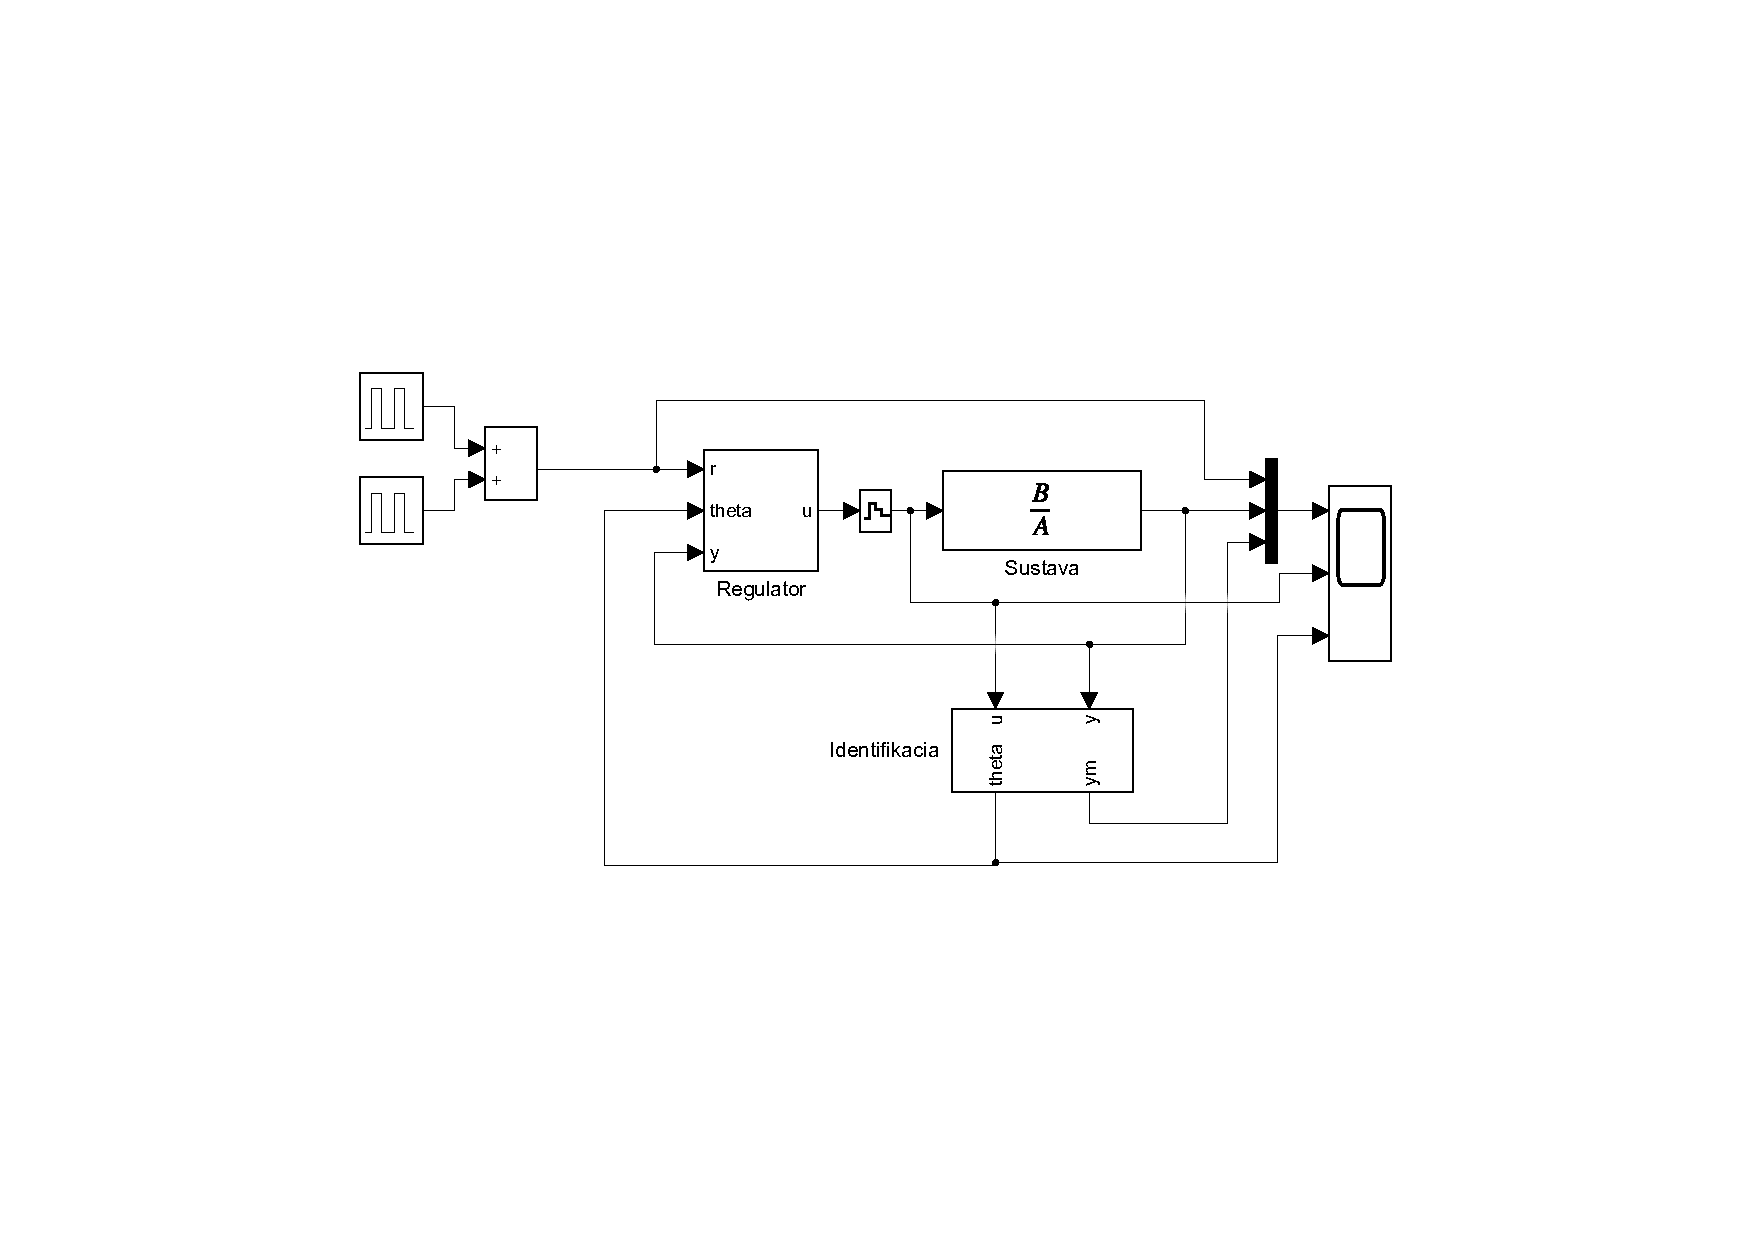
\includegraphics[viewport=55mm 60mm 236mm 150mm, clip, scale=0.9]{ar03_sim_RST.pdf}
	}

    \vspace{-2mm}

    \figcaption{}

    \vspace{2mm}

    \label{ar03_sim_RST}

\end{centering}

Pred spustením schémy (v Simulinku) je samozrejme potrebné inicializovať parametre riadeného systému (sústavy) a ako sa ukáže aj iné veci (v tomto prípade). Je to realizované v skripte:
{\catcode`\-=12
\lstinputlisting[language=Matlab,
                 caption={Súbor \lstinline{ar03_spustima_STR.m}},
                 % label={vypk01},
                 ]{../../ML/ar03_spustima_STR.m}
}



\noindent
Blok Identifikácia je realizovaný ako na obr.~\ref{Identifikacia} a používa funkciu:
{\catcode`\-=12
\lstinputlisting[language=Matlab,
                 caption={Súbor \lstinline{MNSvRST.m}},
                 % label={vypk01},
                 ]{../../ML/MNSvRST.m}
}



\noindent
Blok Regulátor je realizovaný nasledovne:

\begin{centering}

	\makebox[\textwidth][c]{%
	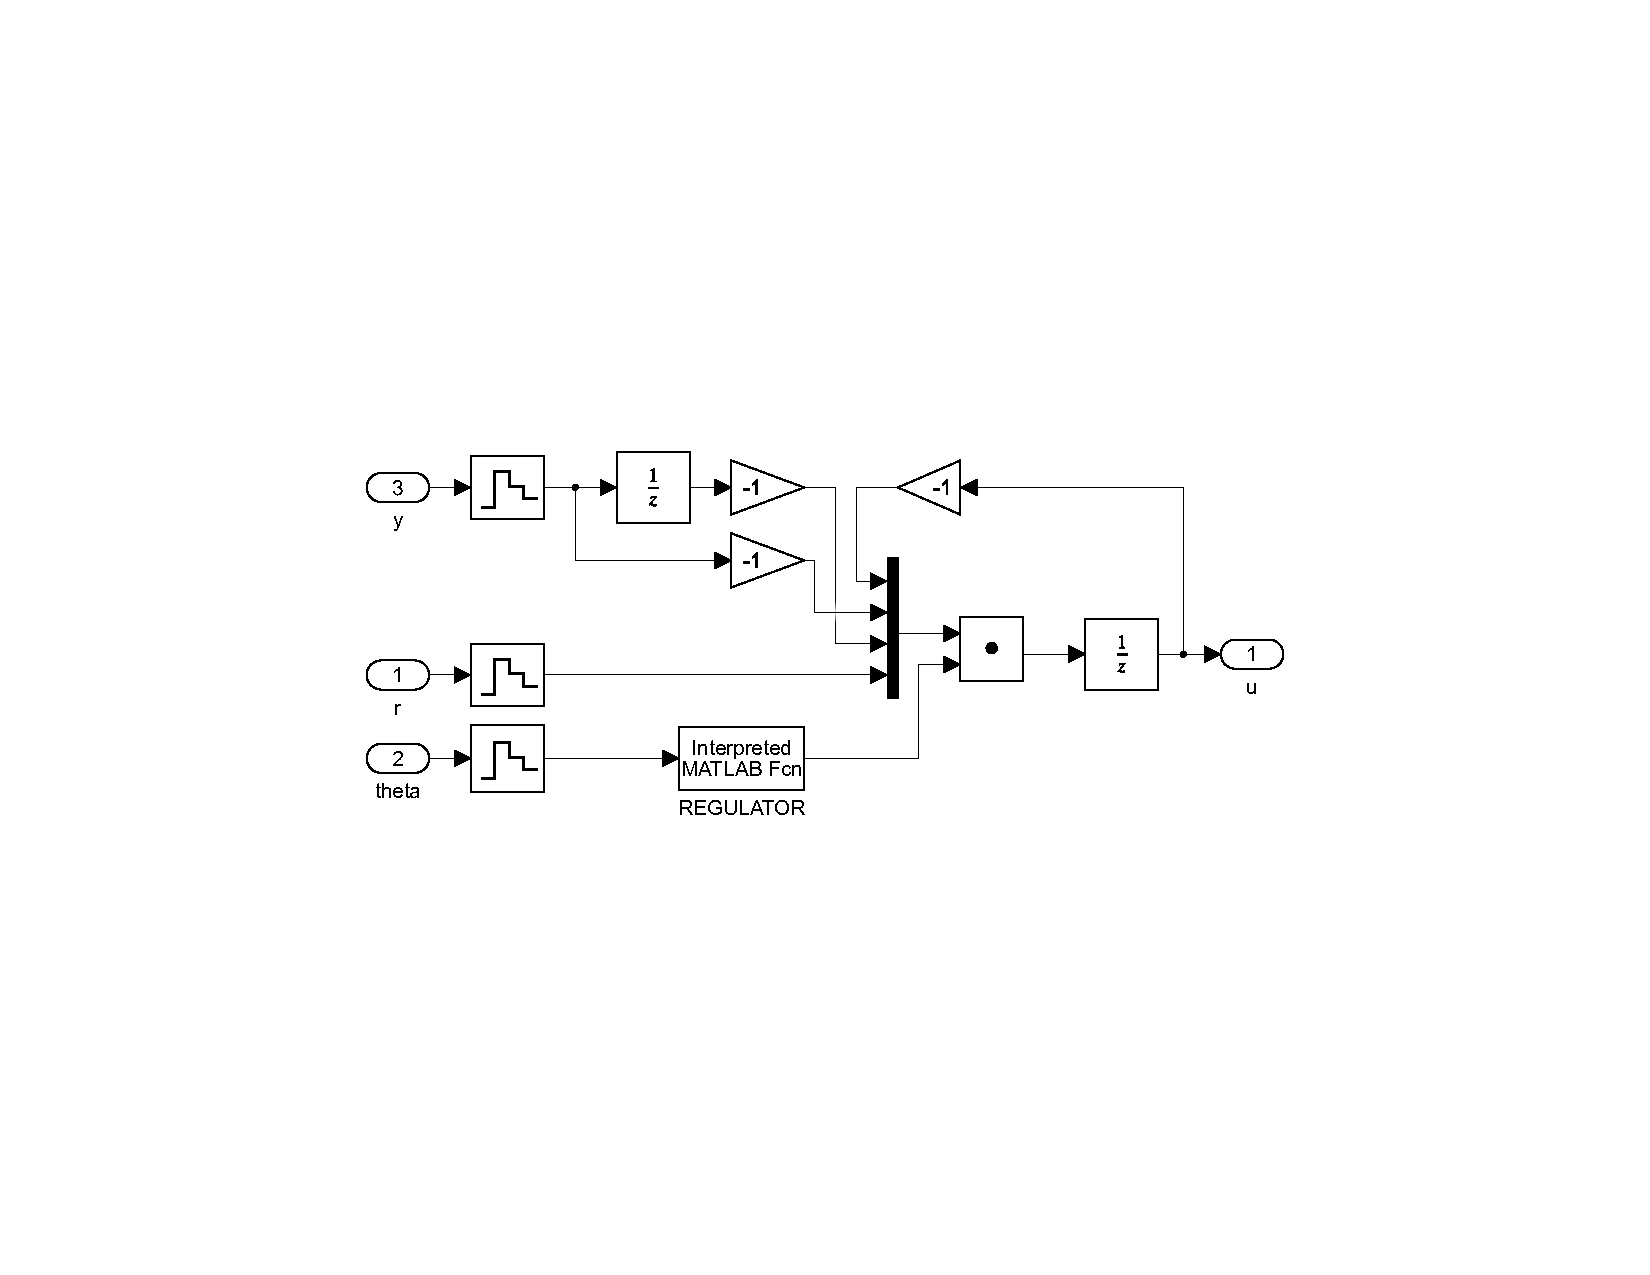
\includegraphics[viewport=60mm 73mm 220mm 145mm, clip, scale=0.9]{Regulator.pdf}
	}

    \vspace{-2mm}

    \figcaption{}

    \vspace{2mm}

    \label{Regulator}

\end{centering}


\noindent
Funkcia, ktorú používa blok Regulátor je nasledovná:

{\catcode`\-=12
\lstinputlisting[language=Matlab,
                 caption={Súbor \lstinline{REGULATOR.m}},
                 % label={vypk01},
                 ]{../../ML/REGULATOR.m}
}












% \newpage

% \vfill

\section{Otázky a úlohy}



\begin{enumerate}[leftmargin=0pt, labelsep=4mm, itemsep=0pt]

	\item Stručne vysvetlite princíp rekurzívnej metódy najmenších štvorcov.

	\item Napíšte Gaussov vzorec a podrobne vysvetlite jednotlivé prvky

	\item Vyjadrite ARX model v tvare diskrétnej prenosovej funkcie alebo v tvare diferenčnej rovnice.

	\item Odvoďte Gaussov vzorec a ukážte, že nájdený extrém je minimum.

	\item Aké (ktoré) prvky obsahuje signálny vektor pri priebežnej identifikácii metódou najmenších štvorcov? (Čo tvorí prvky signálneho vektora pri priebežnej identifikácii metódou najmenších štvorcov?)




	\item Modelom riadeného systému je ARX model. Zákon riadenia má tvar $R(z^{-1}) u(k) =  T(z^{-1}) r(k) -  S(z^{-1}) y(k)$. Nájdite charakteristický polynóm URO.

	\item Modelom riadeného systému je ARX model. Zákon riadenia má tvar $ u(k) =  \Delta u(k) / (1 - z^{-1})$, kde
	\begin{equation*}
		\Delta u(k) = \frac{S(z^{-1})}{R(z^{-1})} (r(k) - y(k))
	\end{equation*}
		Nájdite charakteristický polynóm URO.

	\item Stručne vysvetlite výpočet parametrov regulátora metódou pole-placement.

	\item Vysvetlite podstatu metód návrhu polynómu $T(z^{-1})$ pri STR.


\end{enumerate}

















\end{document}
